%%%%%%%%%%%%%%%%%%%%%%%%%%%%%%%%%%%%%%%%%%%%%%%%%%%%%%%%%%%%%%%%%%%%%
%% This is a (brief) model paper using the achemso class
%% The document class accepts keyval options, which should include
%% the target journal and optionally the manuscript type. 
%%%%%%%%%%%%%%%%%%%%%%%%%%%%%%%%%%%%%%%%%%%%%%%%%%%%%%%%%%%%%%%%%%%%%
\documentclass[journal=jacsat,manuscript=article]{achemso}
\SectionNumbersOn
%\usepackage[letterpaper,left=0.5in,right=0.5in,top=1.0in,bottom=1.0in]{geometry}

%%%%%%%%%%%%%%%%%%%%%%%%%%%%%%%%%%%%%%%%%%%%%%%%%%%%%%%%%%%%%%%%%%%%%
%% Place any additional packages needed here.  Only include packages
%% which are essential, to avoid problems later. Do NOT use any
%% packages which require e-TeX (for example etoolbox): the e-TeX
%% extensions are not currently available on the ACS conversion
%% servers. 
%%%%%%%%%%%%%%%%%%%%%%%%%%%%%%%%%%%%%%%%%%%%%%%%%%%%%%%%%%%%%%%%%%%%%
\usepackage[version=3]{mhchem} % Formula subscripts using \ce{}
\usepackage{siunitx} % generating degrees Celsius in the document 
\usepackage{color}
\usepackage{soul} % allows highlighting text 
\usepackage{makecell}
\usepackage{booktabs}
\usepackage{amsmath}
\usepackage{amssymb}
\usepackage{todonotes}
\usepackage{gensymb}
\usepackage{verbatim}
\usepackage{hyperref}
\hypersetup{
    colorlinks=true,
    citecolor= red,
    linkcolor=blue,
    urlcolor=blue, 
    breaklinks=true
}
\usepackage{ulem}
\usepackage{float}


%%%%%%%%%%%%%%%%%%%%%%%%%%%%%%%%%%%%%%%%%%%%%%%%%%%%%%%%%%%%%%%%%%%%%
%% If issues arise when submitting your manuscript, you may want to
%% un-comment the next line.  This provides information on the
%% version of every file you have used.
%%%%%%%%%%%%%%%%%%%%%%%%%%%%%%%%%%%%%%%%%%%%%%%%%%%%%%%%%%%%%%%%%%%%%
%%\listfiles

%%%%%%%%%%%%%%%%%%%%%%%%%%%%%%%%%%%%%%%%%%%%%%%%%%%%%%%%%%%%%%%%%%%%%
%% Place any additional macros here.  Please use \newcommand* where
%% possible, and avoid layout-changing macros (which are not used
%% when typesetting).
%%%%%%%%%%%%%%%%%%%%%%%%%%%%%%%%%%%%%%%%%%%%%%%%%%%%%%%%%%%%%%%%%%%%%
\newcommand*\mycommand[1]{\texttt{\emph{#1}}}
\DeclareRobustCommand
  \Compactcdots{\mathinner{\cdotp\mkern-2mu\cdotp\mkern-2mu\cdotp}}

%%%%%%%%%%%%%%%%%%%%%%%%%%%%%%%%%%%%%%%%%%%%%%%%%%%%%%%%%%%%%%%%%%%%%
%% Meta-data block
%% ---------------
%% Each author should be given as a separate \author command.
%%
%% Corresponding authors should have an e-mail given after the author
%% name as an \email command. Phone and fax numbers can be given
%% using \phone and \fax, respectively; this information is optional.
%%
%% The affiliation of authors is given after the authors; each
%% \affiliation command applies to all preceding authors not already
%% assigned an affiliation.
%%
%% The affiliation takes an option argument for the short name.  This
%% will typically be something like "University of Somewhere".
%%
%% The \altaffiliation macro should be used for new address, etc.
%% On the other hand, \alsoaffiliation is used on a per author basis
%% when authors are associated with multiple institutions.
%%%%%%%%%%%%%%%%%%%%%%%%%%%%%%%%%%%%%%%%%%%%%%%%%%%%%%%%%%%%%%%%%%%%%
\author{Stephen P. Vicchio}
\affiliation[Clemson University]
{Department of Chemical and Biomolecular Engineering, Clemson University, Clemson, SC}
\author{Zhihengyu Chen}
\affiliation[Stony Brook University]
{Department of Chemistry, Stony Brook University, Stony Brook, NY}
\author{Karena Chapman}
\email{karena.chapman@stonybrook.edu}
\affiliation[Stony Brook University]
{Department of Chemistry, Stony Brook University, Stony Brook, NY}
\author{Rachel B. Getman}
\email{rgetman@clemson.edu}
\affiliation[Clemson University]
{Department of Chemical and Biomolecular Engineering, Clemson University, Clemson, SC}

%%%%%%%%%%%%%%%%%%%%%%%%%%%%%%%%%%%%%%%%%%%%%%%%%%%%%%%%%%%%%%%%%%%%%
%% The document title should be given as usual. Some journals require
%% a running title from the author: this should be supplied as an
%% optional argument to \title.
%%%%%%%%%%%%%%%%%%%%%%%%%%%%%%%%%%%%%%%%%%%%%%%%%%%%%%%%%%%%%%%%%%%%%
\title[manuscript]{
Identifying the structure and composition of \ce{Ni(II)}-hydroxo catalyst supported the NU-1000 metal-organic framework
}

%%%%%%%%%%%%%%%%%%%%%%%%%%%%%%%%%%%%%%%%%%%%%%%%%%%%%%%%%%%%%%%%%%%%%
%% Some journals require a list of abbreviations or keywords to be
%% supplied. These should be set up here, and will be printed after
%% the title and author information, if needed.
%%%%%%%%%%%%%%%%%%%%%%%%%%%%%%%%%%%%%%%%%%%%%%%%%%%%%%%%%%%%%%%%%%%%%
\abbreviations{IR,NMR,UV}
\keywords{American Chemical Society, \LaTeX}

%%%%%%%%%%%%%%%%%%%%%%%%%%%%%%%%%%%%%%%%%%%%%%%%%%%%%%%%%%%%%%%%%%%%%
%% The manuscript does not need to include \maketitle, which is
%% executed automatically.
%%%%%%%%%%%%%%%%%%%%%%%%%%%%%%%%%%%%%%%%%%%%%%%%%%%%%%%%%%%%%%%%%%%%%
\begin{document}

%%%%%%%%%%%%%%%%%%%%%%%%%%%%%%%%%%%%%%%%%%%%%%%%%%%%%%%%%%%%%%%%%%%%%
%% The "tocentry" environment can be used to create an entry for the
%% graphical table of contents. It is given here as some journals
%% require that it is printed as part of the abstract page. It will
%% be automatically moved as appropriate.
%%%%%%%%%%%%%%%%%%%%%%%%%%%%%%%%%%%%%%%%%%%%%%%%%%%%%%%%%%%%%%%%%%%%%
%\begin{tocentry}
%
%Some journals require a graphical entry for the Table of Contents.
%This should be laid out ``print ready'' so that the sizing of the
%text is correct.
%
%Inside the \texttt{tocentry} environment, the font used is %Helvetica
%8\,pt, as required by \emph{Journal of the American Chemical
%Society}.
%
%The surrounding frame is 9\,cm by 3.5\,cm, which is the maximum
%permitted for  \emph{Journal of the American Chemical Society}
%graphical table of content entries. The box will not resize if the
%content is too big: instead it will overflow the edge of the box.
%
%This box and the associated title will always be printed on a
%separate page at the end of the document.
%
%\end{tocentry}

%%%%%%%%%%%%%%%%%%%%%%%%%%%%%%%%%%%%%%%%%%%%%%%%%%%%%%%%%%%%%%%%%%%%%
%% The abstract environment will automatically gobble the contents
%% if an abstract is not used by the target journal.
%%%%%%%%%%%%%%%%%%%%%%%%%%%%%%%%%%%%%%%%%%%%%%%%%%%%%%%%%%%%%%%%%%%%%
\begin{abstract}
Heterogeneous catalysts exhibit dynamic changes in composition and structure as a function of environmental conditions that have a profound effect on catalytic performance. For traditional bulk metal heterogeneous catalysts, general trends between composition/structure and function are well established. However, single-site heterogeneous catalysts (SSHCs) where the active site consists of small metal clusters anchored to a solid support the same trends remain undefined. One such SSHC involves a 3d transition metal complex (i.e., \ce{Ni_4O_xH_y}) supported on a porous metal-organic framework (MOF). Herein, we investigate the ligand environment of a \ce{Ni4} cluster supported on the NU-1000 MOF when exposed to reducing conditions (\ce{H2} gas), with the ligand environment varying from \ce{O}, \ce{OH}, \ce{H2O}, and \ce{H} ligands coordinated to the \ce{Ni} atoms. Differential pair distribution functions (dPDF) analysis and \textit{ab initio} thermodynamic analysis probe potential ligand environments of the \ce{Ni_4O_xH_y} cluster. We generate over 300 different structures featuring different \ce{Ni4} clusters (i.e., different ligand environments) while also accounting for the spin states of the \ce{Ni} atoms. Phase diagrams show the relative location of thermodynamically relevant conditions as a function of \ce{H2} and \ce{H2O} chemical potential terms, and dPDF analysis enables comparisons in local structural information to experimental data. Structures with \ce{Ni-O} coordination numbers closer to experimental data occur at high \ce{H2O} chemical potentials, suggesting a large \ce{H2O} chemical potential is present within the MOF. Reasonable agreement is seen in the \ce{Ni-O} peak between model and experimental dPDFs; however, model structures fail to recreate the split \ce{Ni{\Compactcdots}Ni} peaks. Furthermore, dPDF analysis suggests that asymmetric ligand environments in structures containing high \ce{Ni-O} coordination demonstrate features that are most closely related to the experimental structure, such as the \ce{Ni-O} peak and the split \ce{Ni{\Compactcdots}Ni} peaks. The combined modeling approach demonstrates how the SSHC active site structure is sensitive to the environment conditions, and provide insights into the correct coordination environment of the \ce{Ni4} cluster supported on the NU-1000 MOF thereby establish general trends in the \ce{Ni} ligand environment for these heterogeneous catalytic systems.

\end{abstract}

%%%%%%%%%%%%%%%%%%%%%%%%%%%%%%%%%%%%%%%%%%%%%%%%%%%%%%%%%%%%%%%%%%%%%
%% Start the main part of the manuscript here.
%%%%%%%%%%%%%%%%%%%%%%%%%%%%%%%%%%%%%%%%%%%%%%%%%%%%%%%%%%%%%%%%%%%%%

\section{Introduction}
%%%%%%%%%%%%%%%%%%%%%%%%%%%%%%%%%%%%%%%%%%%%%%%%%%%%%%%%%%%%%%%%%%%%%
%% Introduction
%%%%%%%%%%%%%%%%%%%%%%%%%%%%%%%%%%%%%%%%%%%%%%%%%%%%%%%%%%%%%%%%%%%%%

Single-site heterogeneous catalysts (SSHCs) contain well-defined, atomically dispersed active sites that are anchored to solid supports\cite{Hlatky2000, Kaiser2020, Thomas2005, Wasson2019} such as metal-organic frameworks (MOFs),\cite{Zheng2019, AbdelMageed2019, Huang2019} covalent-organic frameworks (COFs),\cite{Zhong2019, Romero-Muniz2020} zeolites,\cite{Mao2016, Kistler2014} and metal\cite{Patel2019, Pei2017, Jiao2019} and metal oxide surfaces.\cite{Bo2019, Riley2018, Tang2019} The atomically dispersed atoms are often 3d transition metals,\cite{Manna2016, Beyzavi2015} with the solid support providing a means to improved metal utilization and more well-defined active site structures.\cite{Qiao2011, Cui2017, Yang2013} The metal atoms are anchored to the support either directly (metal-metal bonds) or by organic ligands (e.g., \ce{OH}-ligands), with the attachment dependent on the type of support. In some cases, the ligand environments may be simialr to homogeneous catalysts.\cite{Rogge2017} Also similar to homogeneous catalysts, active site structures for SSHCs are unique, which makes SSHCs appealing for carrying out challenging chemistries since they can be tuned to improve catalytic activity and selectivity.

Designing SSHCs requires developing structure-function relationships between catalyst composition and structure with performance. The structures of SSHCs are strongly influenced by environmental conditions (e.g., $T$, $p$), for example, inducing changes in coordinating ligands and structural environments, e.g., by promoting metal atom sintering.\cite{Kim2015,Redfern2018,Mian2020,Li2016sintering,Ye2017,Halder2020,Mian2020,Daelman2019}  Predicting how environmental conditions alter any SSHC is non-trivial due to the uniqueness of SSHCs, and depends on both the metal and the support.  Given catalyst structure drives catalyst function,\cite{DeRita2019} designing SSHCs requires an understanding about the catalyst structure and composition under environmental conditions.\cite{Tang2019} This remains an ongoing challenge, with rational catalyst design inhibited by difficulties in determining the precise active site.

% The downside to this uniqueness is that it complicates catalyst design, since the patterns of behavior that are common with traditional bulk metal catalysts are not present.

% However, the same trends, such as how the ligand environment evolves under different conditions or whether or not the metal centers will agglomerate, does not currently exist for SSHCs. 

% For example, \citeauthor{DeRita2019} demonstrates that local coordination of isolated \ce{Pt} atoms deposited on \ce{TiO2} nanoparticles evolve to \ce{(PtO2)_{ads}} species under mild reduction (250 \degree C in \ce{H2}) and to \ce{(PtOH)_{ads}} species under harsh reduction (450 \degree C in \ce{H2}). These structural changes, as determined by both in situ atomic-resolution microscopy and spectroscopy-based characterization supported by first-principle calculations, strongly influence the chemical reactivity for \ce{CO} oxidation.

% Systematically addressing how the local coordination environment changes in responses to variations in environmental conditions is essential when determining structure-function relationships for SSHCs regardless of the support.

% Similarly, reduction environmental conditions activate a \ce{Ni^{II}}-oxo, hydroxo clusters supported metal complex in a MOFs by altering local \ce{Ni} coordination by manipulating the \ce{H}, \ce{O}, \ce{OH}, \ce{H2O} ligands present.\cite{Li2016sintering,Ye2017} Conversely, certain reduction environmental conditions (i.e., 200 \degree C in \ce{H2}) drive a Copper(II)-hydroxo SSHC supported in a MOFs to encapsulated \ce{Cu^{0}} nanoparticles\cite{Halder2020,Mian2020} by removal of any \ce{OH} and \ce{H2O} ligands present.

In this work, we seek to elucidate the ligand environment of single-site \ce{Ni} catalysts under catalytic operating conditions because of their importance in a variety of reactions, including the Shell higher oligomers process (SHOP),\cite{1988Reuben} \ldots Specifically, we explore a \ce{Ni^{II}} catalyst supported on the MOF NU-1000, a.k.a. Ni@NU-1000.\cite{Mondloch2013} MOFs are porous crystals comprised of metal oxide/hydroxide nodes connected by organic ``linker" molecules. NU-1000 is comprised of \ce{Zr6(\mu_{3}-O)4(\mu_{3}-OH)4(H2O)4(OH)4} nodes connected with tetratopic 1,3,6,8-tetrakis (p-benzoate) pyrene (TBAPy) linkers. Ni supported on NU-1000 has been studied \ldots The Ni ions are known to anchor to the NU-1000 nodes. The structure was initially thought to consist of a single \ce{Ni^{II}} ion coordinated two to three \ce{H2O} ligands, depending on the temperature.\cite{Li2016sintering} However, difference envelope density (DED) analysis of powder diffraction data and electron microscopy later revealed that the catalyst is actually comprised of four \ce{Ni^{II}} ions per node.\cite{PlateroPrats2017} Computational studies by \citeauthor{Ye2017} then suggested that the catalyst is a four ion cluster with oxo and hydroxo ligands that is attached to multiple nodes within NU-1000.\cite{Ye2017} The active site has always been considered to be a Ni hydride, formed upon exposure to \ce{H2} gas.\cite{Li2016sintering,Shabbir2020,Ye2017} For example, in the work by \citeauthor{Ye2017} et al., the catalyst was assumed to be \ldots  However, the precise ligand environment remains to be resolved.\cite{PlateroPrats2017b,Rimoldi2017,Ikuno2017} Addressing questions related to the active site structure are important in improving these Ni-NU-1000 catalysts, and the results will be useful for understanding ligand environments in other 3d transition metal ion catalysts as well. 
 
 %  Similar ligated \ce{Ni} catalysts are now found in heterogeneous systems, such as zeolites\cite{2014Finiels} and MOFs.\cite{Ye2017, Bernales2016}

{\color{red}Fix this paragraph: I edited it before getting through the entire manuscript, so some things are incorrect:} Along these lines, in this work, we explore the ligand environment of a four-ion \ce{Ni^{II}} cluster under conditions relevant to catalytic hydrogenation. Specifically, we use a combination of differential pair distribution function (dPDF) analysis, density functional theory (DFT), and \textit{ab initio} thermodynamic modeling to learn the ligand environment of Ni-NU-1000. We find that the \ce{Ni} coordination environment contains an asymmetric arrangement of \ce{OH}, \ce{H2O}, and \ce{O} ligands and that each Ni ion has a coordination number of XX. Structures that can achieve such high coordination exhibit large chemical potentials of \ce{H2O} even under reducing conditions, suggesting that NU-1000 is able to store \ce{H2O} under these conditions. Notably, we do not identify structures featuring Ni hydrides, which have to date been thought of as being part of the active site in metal@NU-1000 catalysts, in our analysis.    Our results provide insights into the local coordination of the Nickel metal complex that will be useful in hypothesizing and modeling catalytic mechanisms on such catalysts.  

% the \ce{Ni} metal complex ligand environment is sensitive to environmental conditions ($T$, $P_{\text{\ce{H2}}}$, and $P_{\text{\ce{H2O}}}$), and that

\section{Methodology}
%%%%%%%%%%%%%%%%%%%%%%%%%%%%%%%%%%%%%%%%%%%%%%%%%%%%%%%%%%%%%%%%%%%%%
%% Methodology
%%%%%%%%%%%%%%%%%%%%%%%%%%%%%%%%%%%%%%%%%%%%%%%%%%%%%%%%%%%%%%%%%%%%%

\begin{figure}[H]
    \centering
    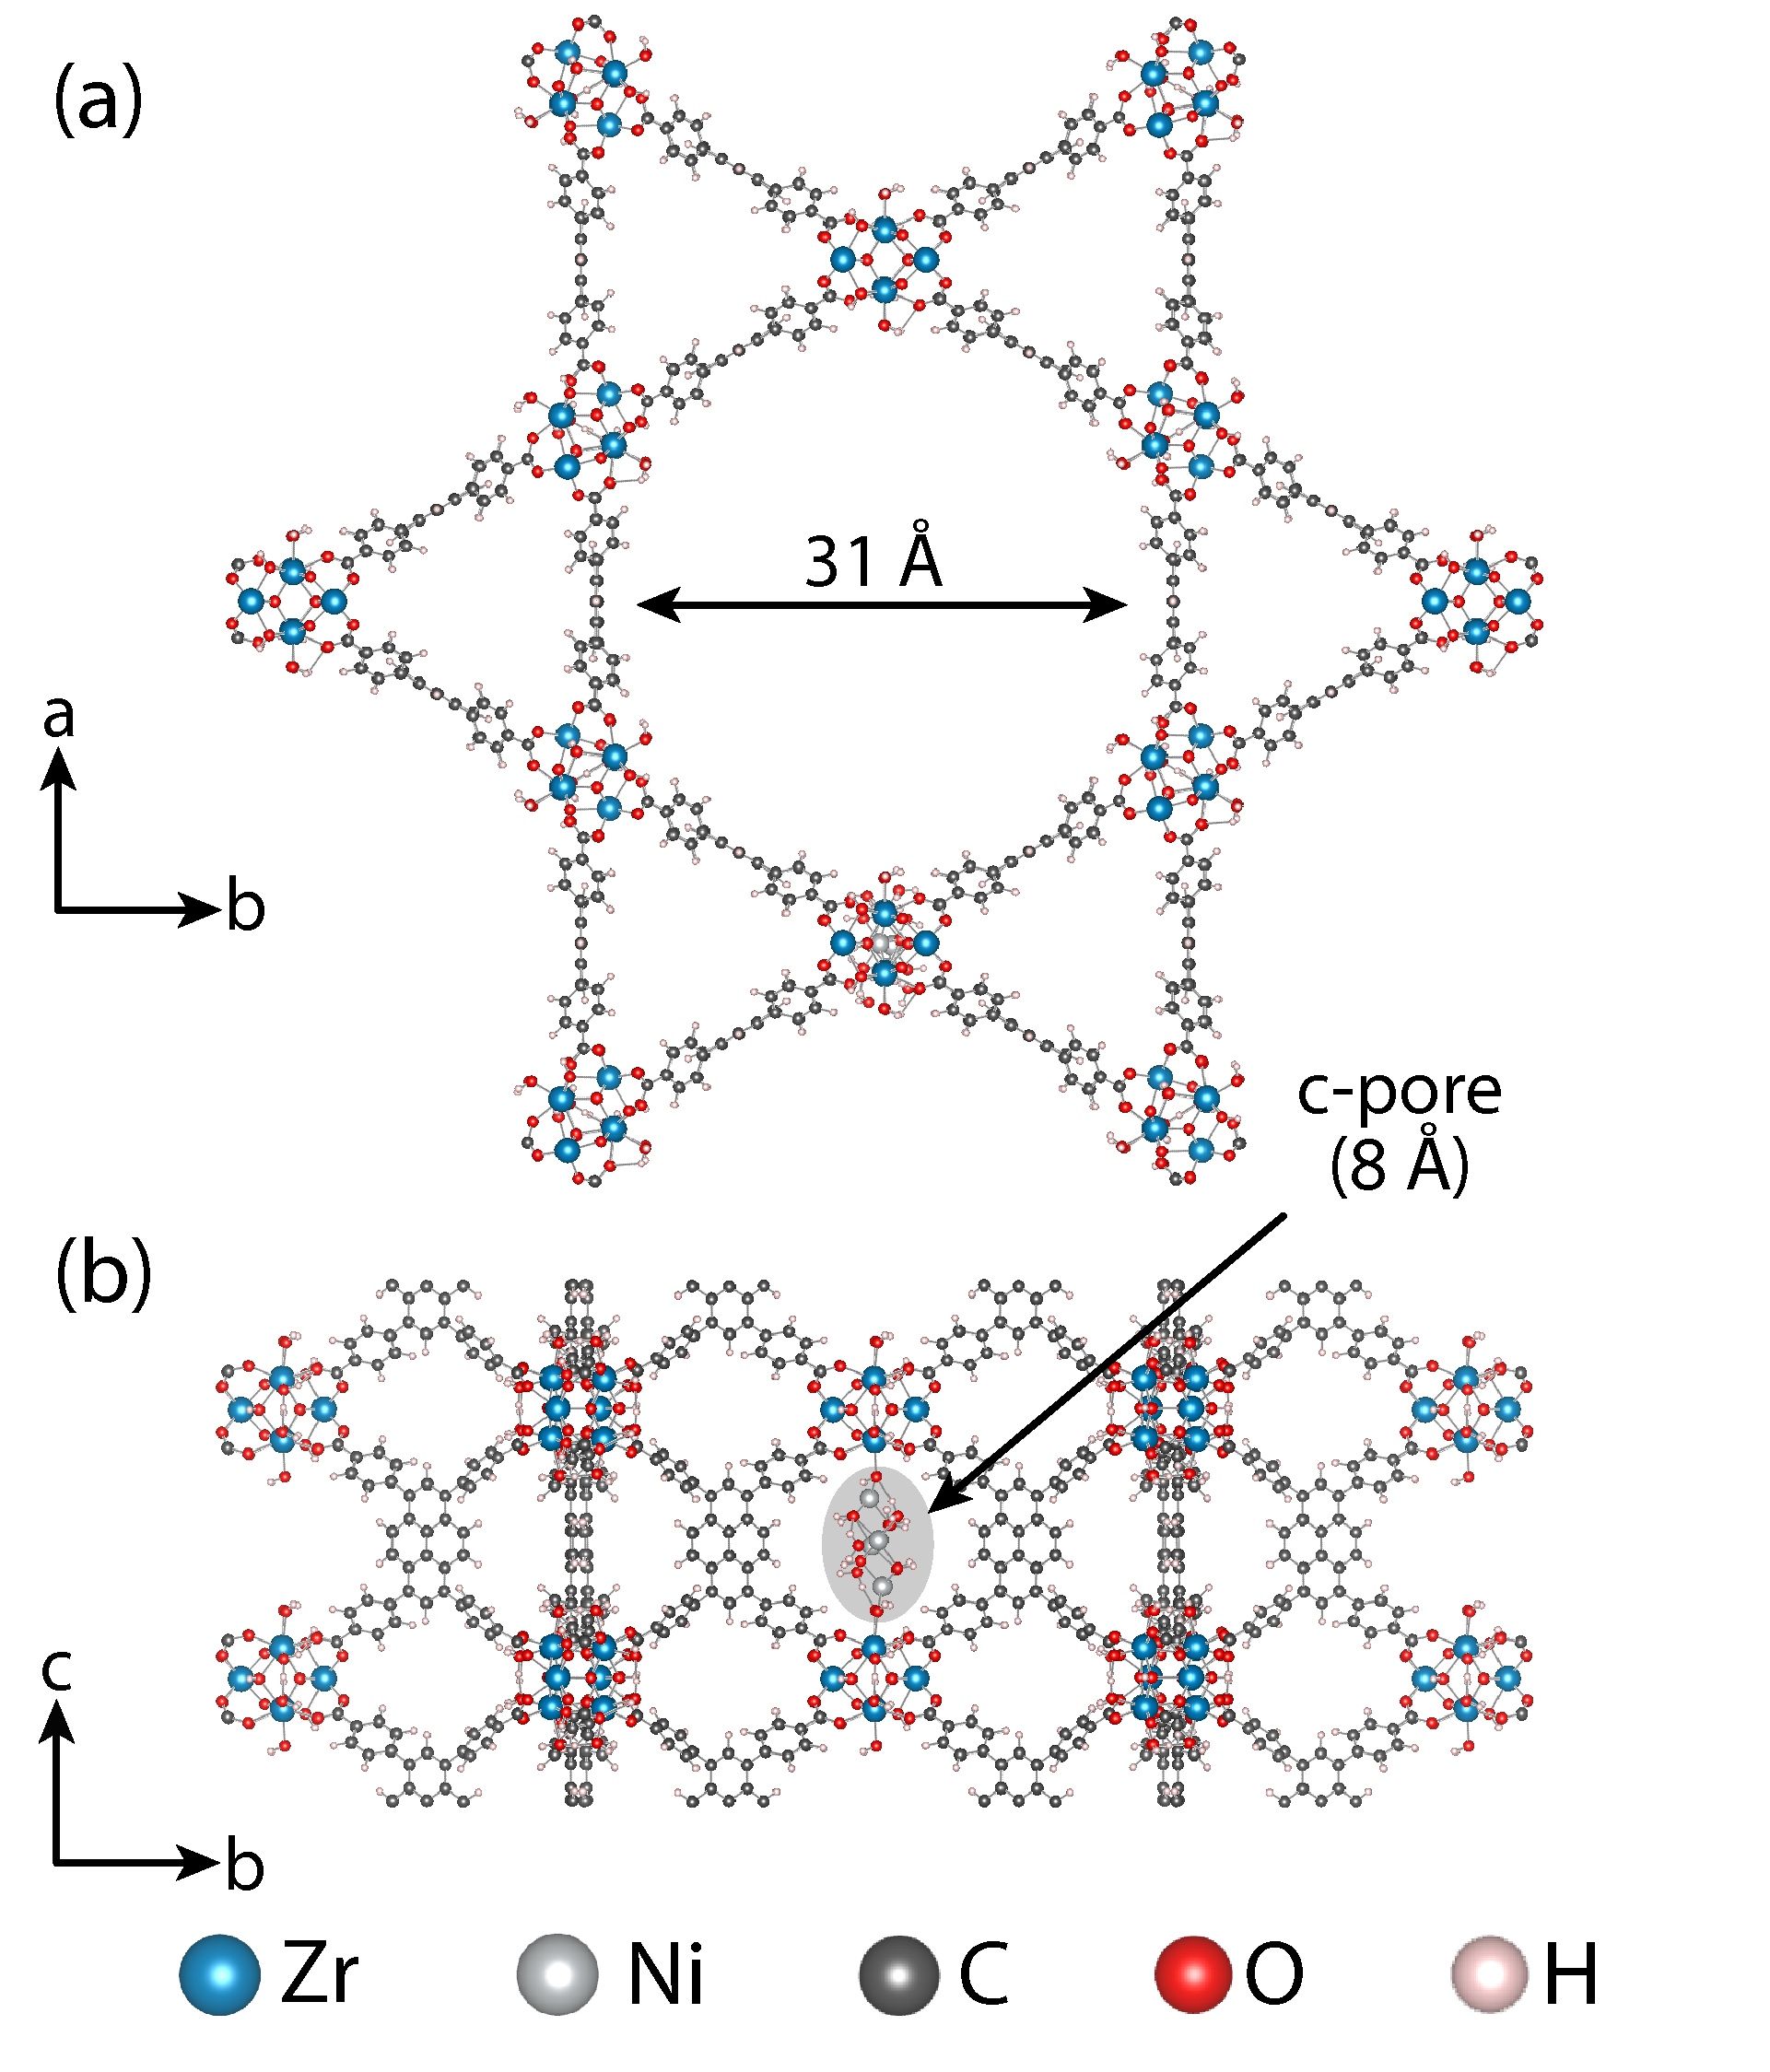
\includegraphics[width=3.0in]{zi-images/00-General-Graphics/2022-figure-MOF-schematic.png}
    \caption{
    The structure of NU-1000 shown along the (a) c-axis and the (b) a-axis with the location of the metal complex location highlighted by the gray oval (shown in  (b)). 
    }
    \label{fig:Ni-MOF-model}
\end{figure}

% The \ce{Ni4} cluster spans the length of the c-pore of NU-1000 ($\sim$10 {\AA}), and is attached to adjacent nodes of the pore.

\subsection{NU-1000 and Hypothetical Catalyst Structure}

NU-1000 has a \ldots structure with \ldots. The full crystal structure is shown in Figure~\ref{fig:Ni-MOF-model}a.  DFT-optimized unit cell parameters are $a=b=40.611$ {\AA}, $c=15.990$ {\AA}, $\alpha=\beta=\ang{90}$, and $\gamma=\ang{60}$.\cite{PlateroPrats2017} Based on the current knowledge about Ni-NU-1000 catalysts, catalyst structures in this work are assumed to comprise four \ce{Ni} ions that span the small (8~\AA) pores in NU-1000 and connect two adjacent nodes (Figure~\ref{fig:Ni-MOF-model}b).\cite{Ortuno2016,PlateroPrats2017} In computational models, one such catalyst structure is included per NU-1000 unit cell. The Ni cluster binds to the nodes by replacing one proton on each node with a Ni ion, following prior work, giving the Ni cluster a formal charge of +2 (and NU-1000 a formal charge of $-$2).

\subsection{Differential Pair Distribution Function Analysis}

dPDF analysis is performed to reveal key interatomic distances in the Ni-NU-1000 catalysts and provide insight into the ligand environment and structure. Ni-NU-1000 catalysts are synthesized as described \ldots. Synthesized catalysts are then exposed to \ce{H2} (3.5\% in \ce{He}) at 200 \degree C for 2 hours and then cooled to 50 \degree C in \ce{H2}.\cite{PlateroPrats2017} Powder X-ray diffraction (XRD) and total scattering data suitable for PDF analysis are then collected at 50 \degree C in \ce{H2}. PDFs are then taken using the PDFgui software; details of these simulations are described in detail elsewhere.\cite{PlateroPrats2017}. PDFs represent the local structure as a histogram of atom-atom distances in the material weighted by the scattering power of the atoms involved. These are used to derive dPDFs by subtracting the PDF measured for NU-1000 from the PDF measured for Ni-NU-1000, to isolate the atom-atom distances that define the \ce{Ni} cluster and its interaction with NU-1000 support. Of interest are the \ce{Ni{\Compactcdots}Ni}, \ce{Ni-O}, and \ce{O{\Compactcdots}O} distances within the cluster and the \ce{Ni{\Compactcdots}Zr} and \ce{Ni{\Compactcdots}O} distances between the cluster and NU-1000. In this notation, atom pairs not directly bonded to each other are denoted with ``${\Compactcdots}$". Given the lower scattering contribution from the \ce{O} atoms compared to \ce{Ni} atoms, \ce{O{\Compactcdots}O} pairs have very low contribution to the measured data and are not calculated. PDFs of the computed structural models are simulated using typical values of instrument and atomic displacement parameters for such materials and then evaluated for their correspondence to the experimental data over XYZ {\AA} range.  

 

\subsection{Simulated Structures}

Simulations are used to provide molecular-level insight into the types of ligand environments that could lead to the experimentally observed dPDFs. Specifically, we modeled \hl{854} different structures, each comprising 4 \ce{Ni} ions and a variety of ligand environments that include hydroxyl (\ce{OH}), water (\ce{H2O}), hydride (\ce{H}), and oxygen (\ce{O}). (Structures comprising fewer than 4 \ce{Ni} ions were also simulated but gave poor agreement with the experimental dPDF; See \hl{Suppporting Information Section XX}.) Three example structures are shown in Figure~\ref{fig:Ni-MOF-structures}. \textbf{\color{red}The full library of structures considered in this work can be accessed on our GitHub page.} 

\begin{figure}[H]
    \centering
    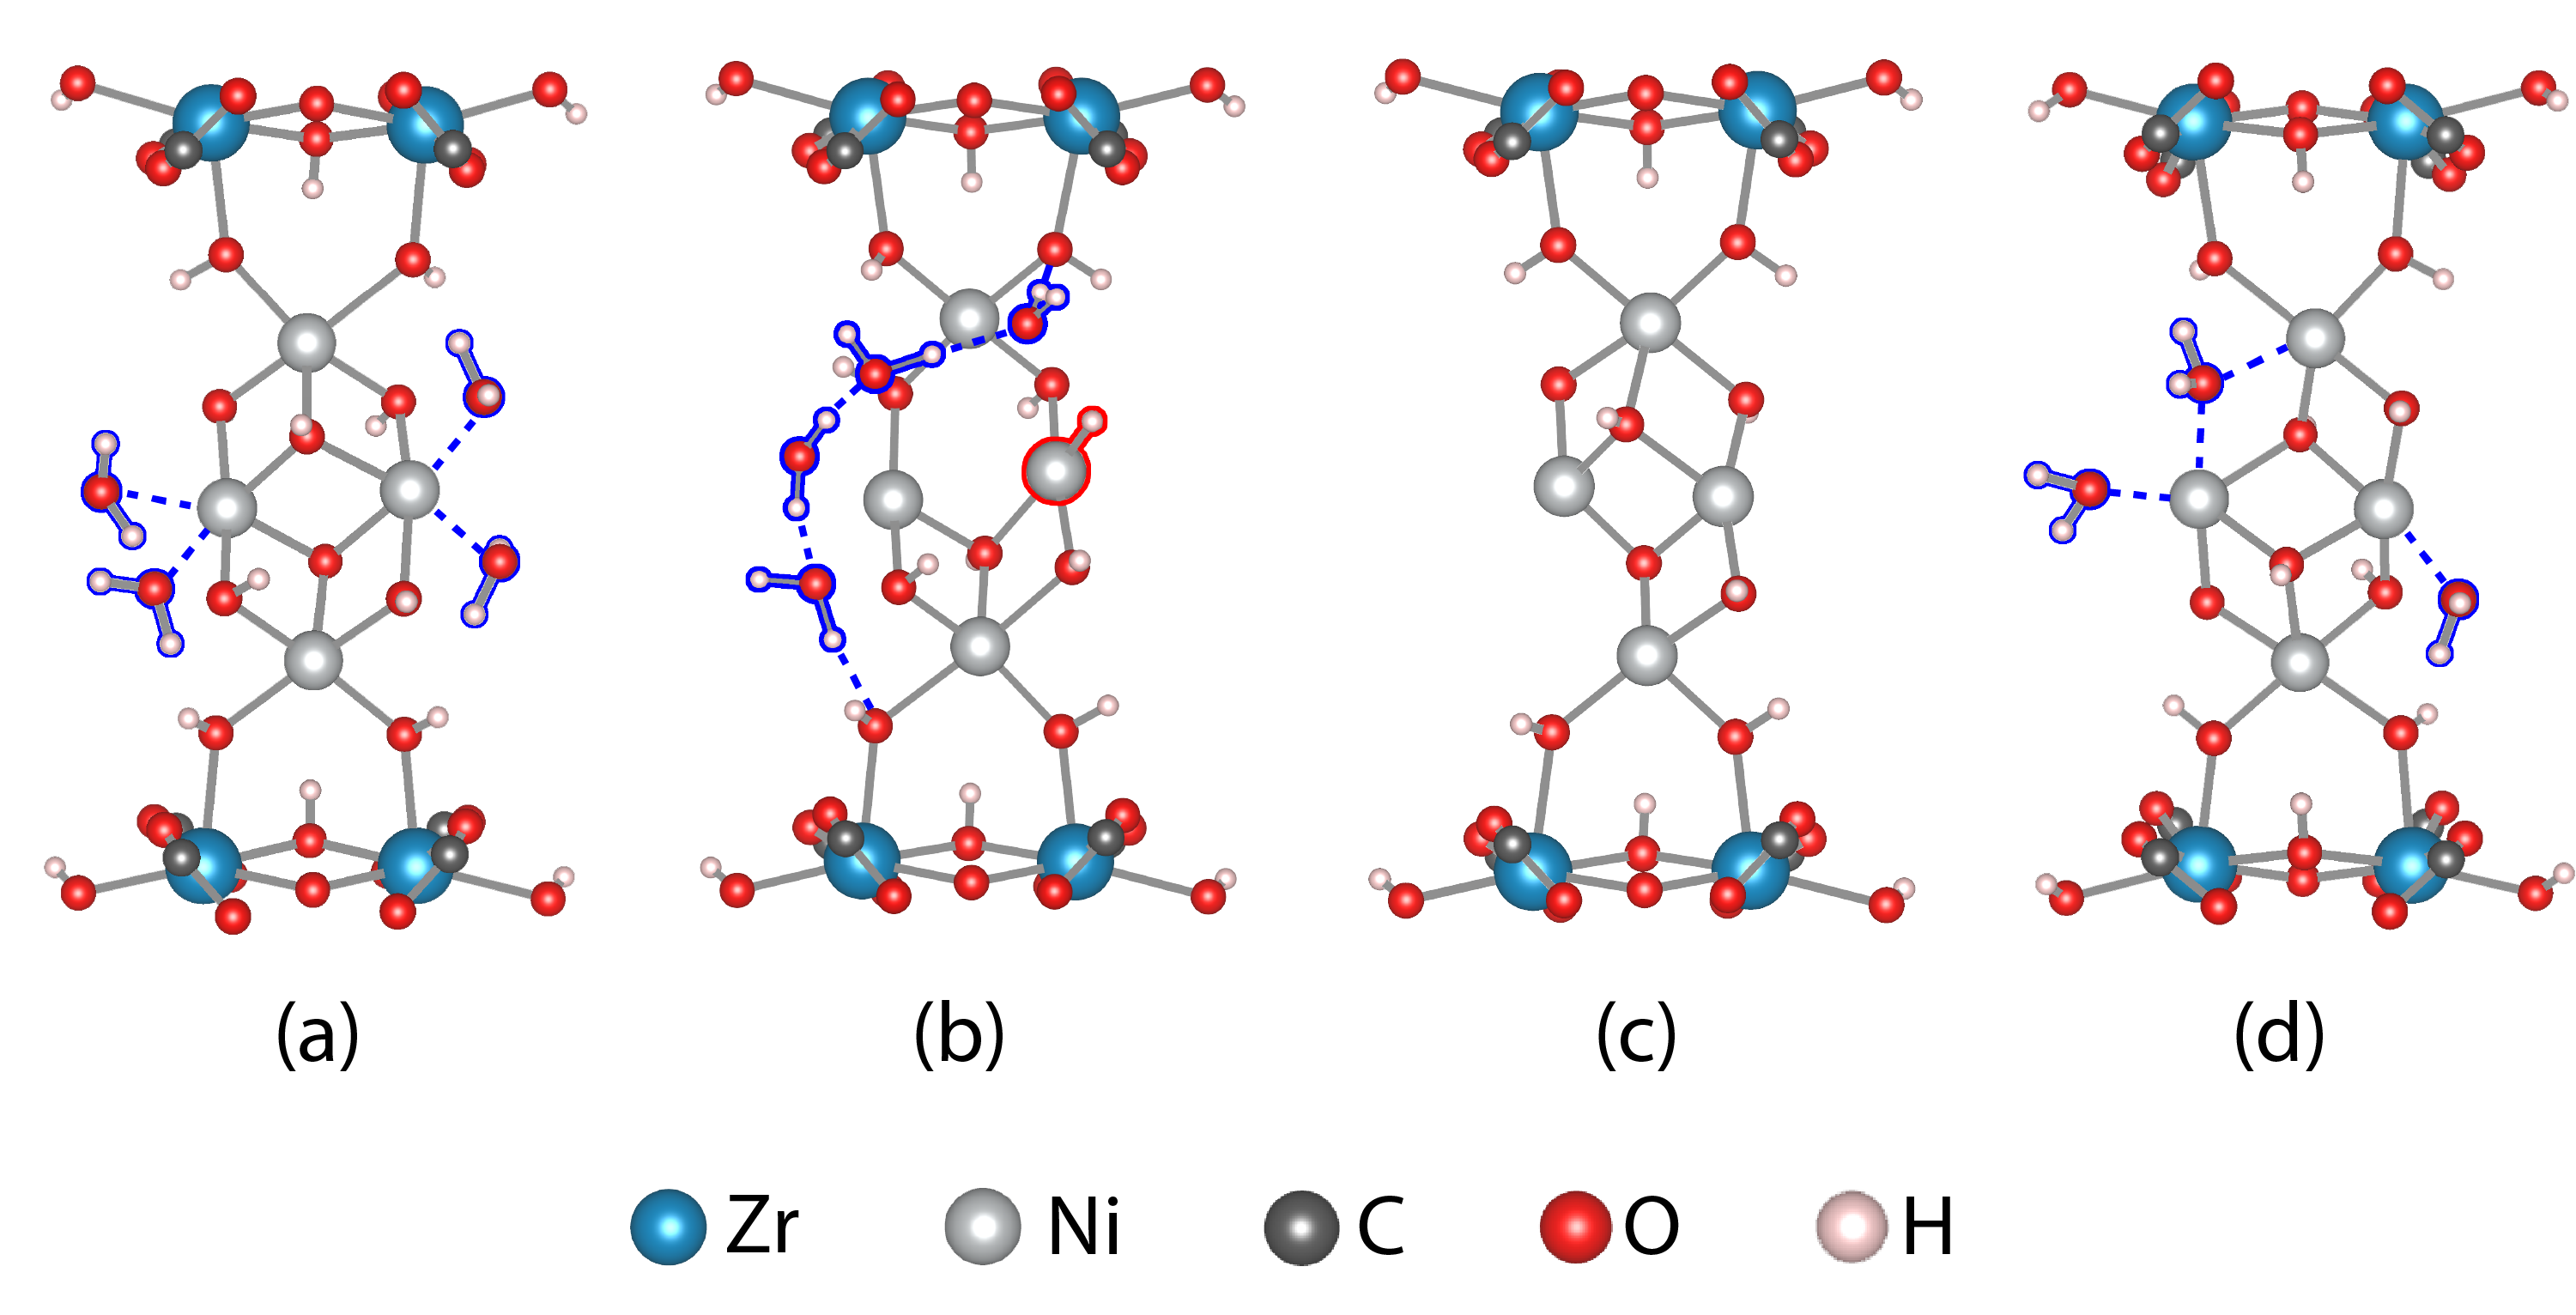
\includegraphics[width=5.0in]{zi-images/00-General-Graphics/2022-figure-clusters-3xstructures.png}
    \caption{
    Different variations of the \ce{Ni} cluster are shown in (a), (b), and (c) with the node of the MOF framework truncated from the renderings. All adsorbed \ce{H2O} molecules are outlined in blue. The diverse ligand \ce{Ni} coordination environments are present with \ce{Ni} coordinating \ce{H2O} and \ce{OH} ligands (all structures), \ce{H} ligands (b), and \ce{O} ligands (c). The reference structure for \textit{ab initio} thermodynamic analysis is shown in (a).
    }
    \label{fig:Ni-MOF-structures}
\end{figure}

\subsection{\textit{ab initio} Thermodynamics Modeling}

\textit{ab initio} thermodynamic analysis\cite{Reuter2003,Reuter2004,Grundner2015,Paolucci2016,Li2016,Getman2008,Mandal2020,Zuo2016,Tang2019} is used to determine the thermodynamically stable structures as functions of chemical potential (which can be related to gas phase temperature and partial pressure using an equation of state; \hl{see Supporting Information} Section XX). We specifically considered the chemical potentials of \ce{H2} and \ce{H2O} because \ldots \ldots The free energy of each structure is then calculated as
\begin{equation}
    \begin{split}
        \Delta F^{(2)}(V,T,\mu_{\text{H}},\mu_{\text{O}},N_{\text{Ni}})  
        & = \Delta F(V,T,N_{\text{H}},N_{\text{O}},N_{\text{Ni}}) - (\mu_{\text{H}})(\Delta N_{\text{H}}) \\
        & - (\mu_{\text{O}})(\Delta N_{\text{O}})  \\ 
    \end{split}
    \label{eq:free-energy-trans}
\end{equation}
where $F$ is the Helmholtz free energy, $V$ is volume, $T$ is temperature, $\mu$ is chemical potential, and $N$ is the number of each type of ligand. The (2) superscript on $F^{(2)}$ indicates the second Legendre transform of $F$,\cite{Alberty1997} i.e., of $N_{\ce{H}}$ and $N_{\ce{O}}$ to $\mu_{\ce{H}}$ and $\mu_{\ce{O}}$. $F$ is equal to $E^\text{elec} + E^\text{ZP} + F^\text{vib}$, where $E^\text{elec}$ is the electronic energy calculated with DFT, $E^\text{ZP}$ is the zero point vibrational energy, and $F^\text{vib}$ is the temperature dependent vibrational free energy. The $\Delta$'s in Eq.~\ref{eq:free-energy-trans} indicate quantities taken relative to a reference structure; the reference structure used in this work is shown in \hl{supporting information Figure SXXX}. 

The chemical potentials of gas phase molecules are calculated as:\cite{Grundner2015}

\begin{equation}
    \mu_{\ce{H}_2(\text{g})}(T,P_{\text{H}_{2}}) = E^\text{elec}_{\text{H}_{2}} + E^\text{ZP}_{\text{H}_{2}} + \Delta \mu_{\text{H}_{2}}(T,P_{\text{H}_{2}})
\end{equation}

% Free energies are calculated assuming equilibrium with an \ce{H2} reservoir to simulate conditions commensurate with catalytic hydrogenation, thus enabling different compositions of \ce{H} to be explored. Further, the structure is also assumed to be in equilibrium with an \ce{H2O} reservoir to account for different \ce{O} content of the cluster (in the form of \ce{O}, \ce{OH}, and \ce{H2O} ligands). 

The \ce{H2O} chemical potential ($\mu_{\ce{H}_2\text{O}(\text{g})}(T,P_{\text{H}_{2}\text{O}})$) is computed analogously. 

% Following these assumptions, $\mu_{\ce{H}} = \frac{1}{2} \mu_{\ce{H}_2(\text{g})}$, $\mu_{\ce{H2O}} = \mu_{\ce{H2O}(\text{g})}$, and $\mu_{\text{O}} = \mu_{\text{H}_2\text{O}} - \mu_{\ce{H2}}$. 

\subsection{Density Functional Theory Calculations}
Electronic energies are calculated using the CP2K software package\cite{Hutter2014} using the PBE exchange and correlation functional\cite{Perdew1996}, damped D3 dispersion corrections,\cite{Grimme2010}, the DZVP-MOLOPT basis set, and Goedecker pseudopotentials.\cite{Goedecker1996} Plane waves are simulated up to 360 Ry. The Unrestricted Kohn-Sham (UKS) method is employed given the open shell natures of the \ce{Ni} ions. As a single \ce{Ni(II)} ion can adopt singlet or triplet states, clusters with four \ce{Ni} ions can adopt singlet, triplet, quintet, septet, or nonet states. We consider all of these spin states for each catalyst structure;\cite{Shabbir2020,Ye2017,Bernales2016,Mandal2020b} spin states exhibiting spin contamination are removed from our analysis (details about how spin contamination is determined and the criteria used to keep or remove structures is provided in Supporting Information Section XX). Electronic energies used in Eq.~\ref{eq:free-energy-trans} are obtained from geometry relaxations where all atoms in the periodic unit cell are allowed to relax. $E^\text{ZP}$ and $F^\text{vib}$ used in Eq.~\ref{eq:free-energy-trans} are calculated from the calculated vibrational modes. At each unique composition, we compute the vibrational modes for structures within 100 kJ/mol of lowest electronic energy structure at that configuration, which reduced the number of structures from 854 to 311 for vibrational mode analysis. Further details about how the vibrational modes were calculated are provided in Supporting Information, along with full descriptions of how $E_{\text{H}_2}$ and $E_{\text{H}_2\text{O}}$ are calculated and sample CP2K input files for all types of DFT calculations carried out in this work. 

 We fix the organic linker and inorganic nodes, thereby only calculating only the \ce{Ni} cluster vibrational contributions to the free energy ($F^\text{vib}$). We ensure that the same atoms are fixed across all frequency calculations in order to correctly compare ($F^\text{vib}$). When constructing the vibrational partition function, all frequencies less than 50 cm\textsuperscript{-1} are replaced with 50 cm\textsuperscript{-1} to correct for the breakdown in the harmonic oscillator approximation for low frequency vibrational modes.\cite{Ribeiro2011} The partitions functions are computed in the pMuTT\cite{LYM2019106864} Python package to compute $E^\text{ZP}$ and $F^\text{vib}$ for all structures. A sample input file for the CP2K frequency calculations is provided in the Supporting Information.

\section{Results and Discussion}
%%%%%%%%%%%%%%%%%%%%%%%%%%%%%%%%%%%%%%%%%%%%%%%%%%%%%%%%%%%%%%%%%%%%%
%% Results 
%%%%%%%%%%%%%%%%%%%%%%%%%%%%%%%%%%%%%%%%%%%%%%%%%%%%%%%%%%%%%%%%%%%%%

% dPDF Diagram
\begin{figure}[H]
    \centering
    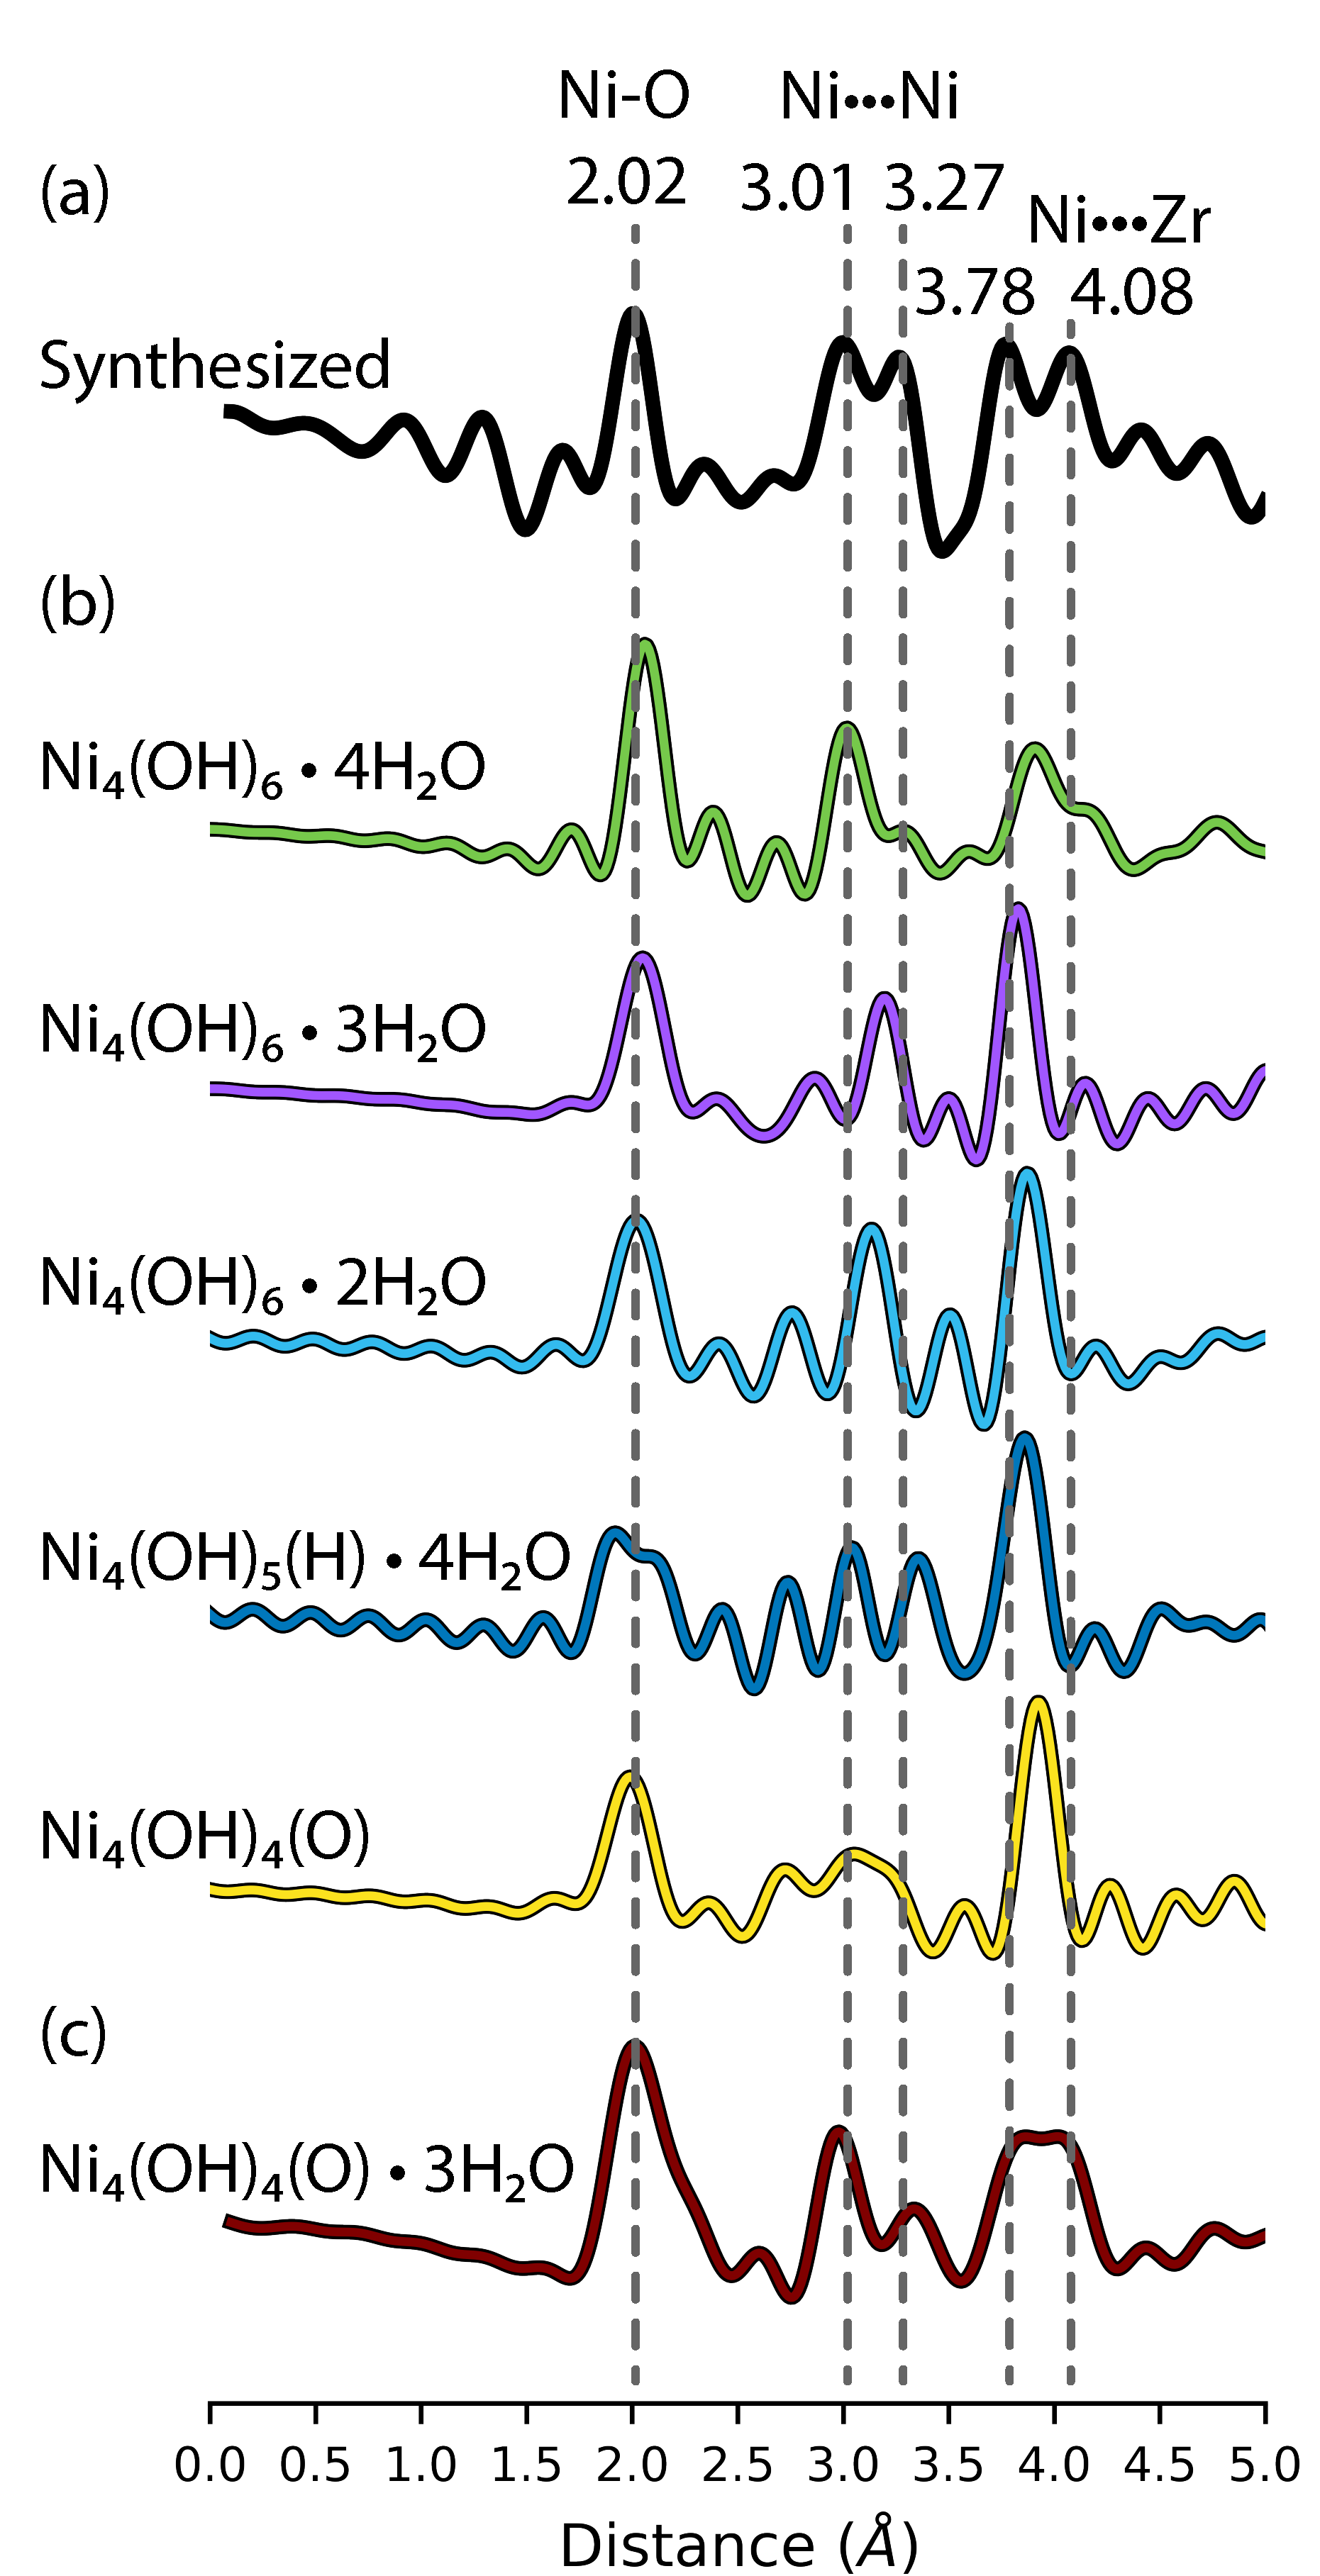
\includegraphics{zi-images/01-Ni-Graphics/2021-MAIN-single-dPDF.png}
    \caption{
    dPDF spectra for the synthesized (a) and simulated (b and c) structures. Structures in b are select thermodynamic minima from \textit{ab initio} thermodynamic analysis, and the structure in c \ldots. The \ce{Ni-O}, \ce{Ni{\Compactcdots}Ni}, and \ce{Ni{\Compactcdots}Zr} distances of the experimental are indicated by the gray dashed lines, enabling comparisons in peak positions between the experimental and model structures. The color scheme is the same as in Figures~\ref{fig:Ni-structure-diagram} and \ref{fig:phase_diagram_Ni}.
    }
    \label{fig:dPDFs-graphic}
\end{figure}

The dPDF spectrum for the synthesized Ni-NU-1000 catalyst is shown in Figure~\ref{fig:dPDFs-graphic} (a).\cite{PlateroPrats2017} Key peaks are the single peak at 2.02 {\AA}, split peaks at 3.01 {\AA} and 3.27 {\AA}, and split peaks at 3.78 {\AA} and 4.08 {\AA} (Figure~\ref{fig:dPDFs-graphic} (a)). These correspond to \ce{Ni-O}, \ce{Ni{\Compactcdots}Ni}, and \ce{Ni{\Compactcdots}Zr} distances, respectively. Figure~\ref{fig:dPDFs-graphic} (a) also indicates that the \ce{Ni-O} coordination number in the Ni-NU-1000 catalyst is $\sim$5. 

To begin to identify the ligand environments that could lead to the observed interatomic distances and \ce{Ni-O} coordination number, we used \textit{ab initio} thermodynamic analysis to identify the thermodynamically most stable structures within our database where the \ce{Ni-O} coordination number is $\sim$5. This data is presented as a phase diagram in Figure~\ref{fig:phase_diagram_Ni}. In the phase diagram in Figure~\ref{fig:phase_diagram_Ni}, the different colored regions correspond to different structures, which are depicted in Figure~\ref{fig:Ni-structure-diagram}. Specifically, these are the structures that minimize $\Delta F^{(2)}$ at the specified values of $\Delta \mu_{\text{H}_2}$ and $\Delta \mu_{\text{H}_2\text{O}}$ (here the $\Delta$'s indicate that these values are taken with respect to the analogous values at 0~K; See \hl{Supporting Information Section XX} for further details). Each colored region is additionally labeled with the \ce{Ni-O} coordination number of the structure. These values span from very small ($\sim$1) to values within the range observed experimentally ($\sim$5). Specifically, structures \ce{Ni4(OH)6.2H2O} (cyan), \ce{Ni4(OH)6.3H2O} (purple), and \ce{Ni4(OH)6.4H2O} (green) give \ce{Ni-O} coordination numbers in line with the experimentally observed value. Notably, achieving such \ce{Ni-O} coordination numbers requires higher (more positive) values of $\Delta \mu_{\text{H}_2\text{O}}$ and lower (more negative) values of $\Delta \mu_{\text{H}_2}$. (Expansion of the phase diagram to higher $\Delta \mu_{\text{H}_2\text{O}}$ and lower $\Delta \mu_{\text{H}_2}$ does not reveal any additional structures or higher coordination numbers; See \hl{Supporting Information Section XX} for further details.) As higher values of chemical potential correspond to larger concentrations (and lower temperatures), this finding suggests that NU-1000 comprises significant \ce{H2O} concentration, even after exposure to \ce{H2}/\ce{He}) at 200 \degree C for 2 hours and measurement in \ce{H2} at 50 \degree C. Similar \ce{H2O} storage properties have been observed \ldots Of interest is the catalyst composition under operating conditions. As the precise value of \ce{H2O} chemical potential within NU-1000 cannot be known, Figure~\ref{fig:phase_diagram_Ni} includes vertical dashed white line, which indicates the \ce{H2} chemical potential at the measurement conditions of \ce{H2} (3.5\% in \ce{He}) at 50 \degree C. Indeed, two structures along this line exhibit \ce{Ni-O} coordination numbers in agreement with those observed experimentally.       

% Phase Diagram
\begin{figure}[H]
    \centering
    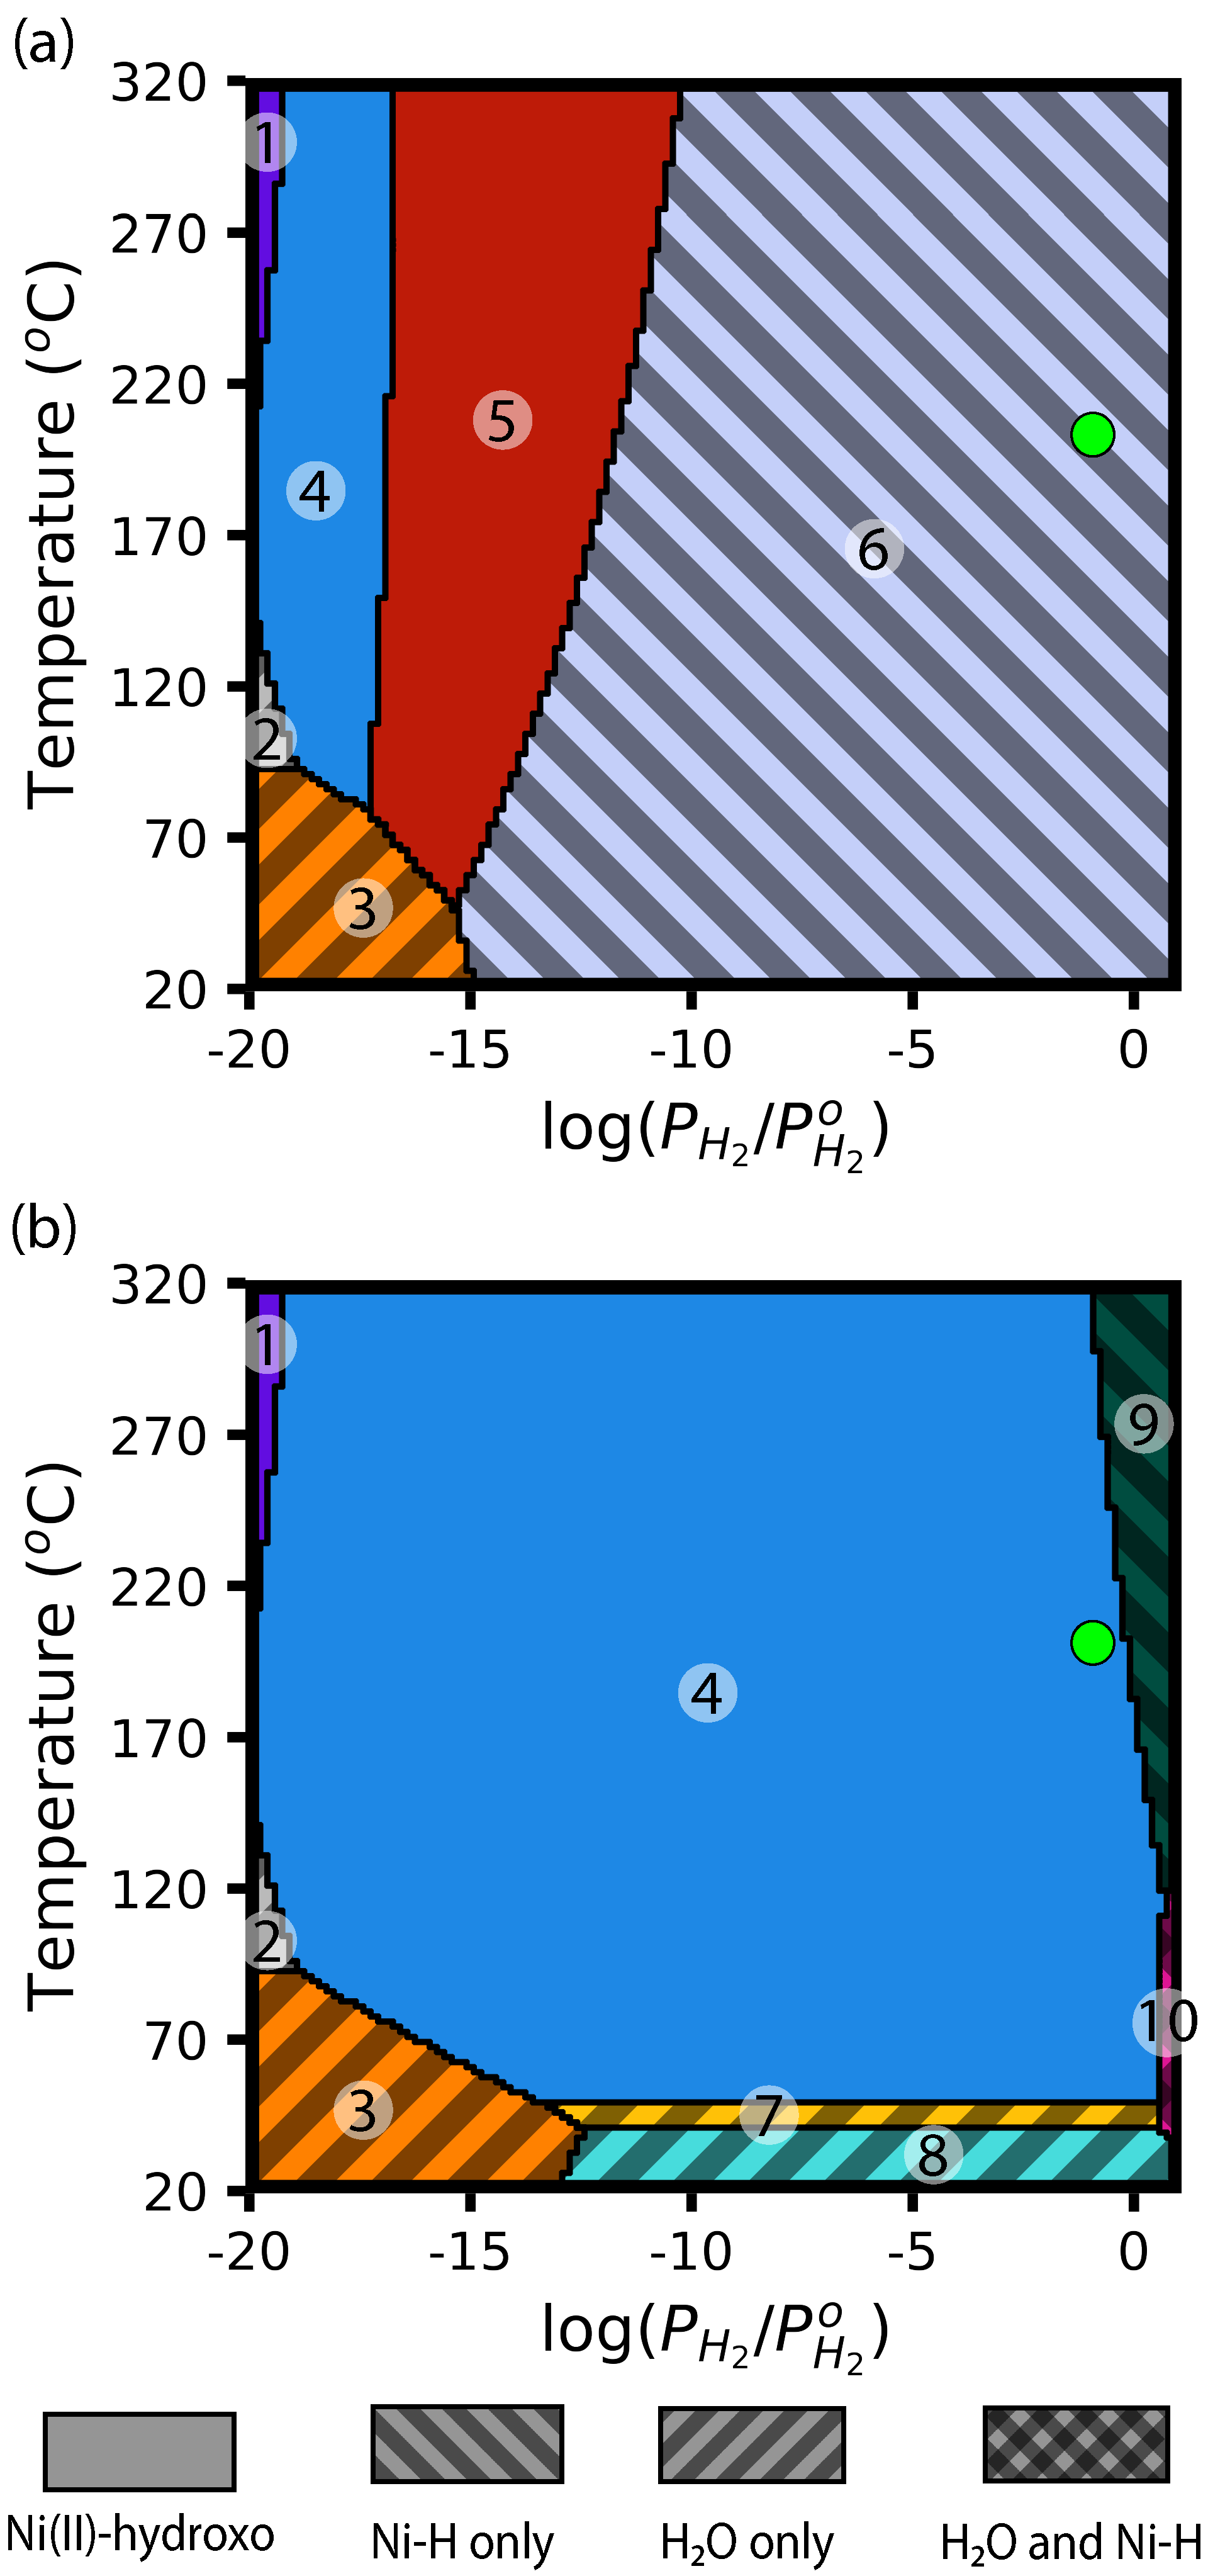
\includegraphics{zi-images/01-Ni-Graphics/2021-MAIN-phase-diagram-combined.png}
    \caption{
    Phase diagram for the \ce{Ni} cluster calculated as a function of $\Delta \mu_{\text{H}_{2}}(T,P_{\text{H}_{2}})$ and $\Delta \mu_{\text{H}_{2}\text{O}}(T,P_{\text{H}_{2}\text{O}})$. The different structures are represented by the different colored regions, with follow the same color scheme as previous figures. {\color{red}EXPLAIN WHAT THE HASHES MEAN}. The vertical white dashed line indicates the value of $\Delta \mu_{\text{H}_2}$ corresponding to the conditions where experimental measurements were taken (\ce{H2} in 3.5\% in \ce{He} at 50 \degree C). 
    }
    \label{fig:phase_diagram_Ni}
\end{figure}  

% Structure Diagram
\begin{figure}[H]
    \centering
    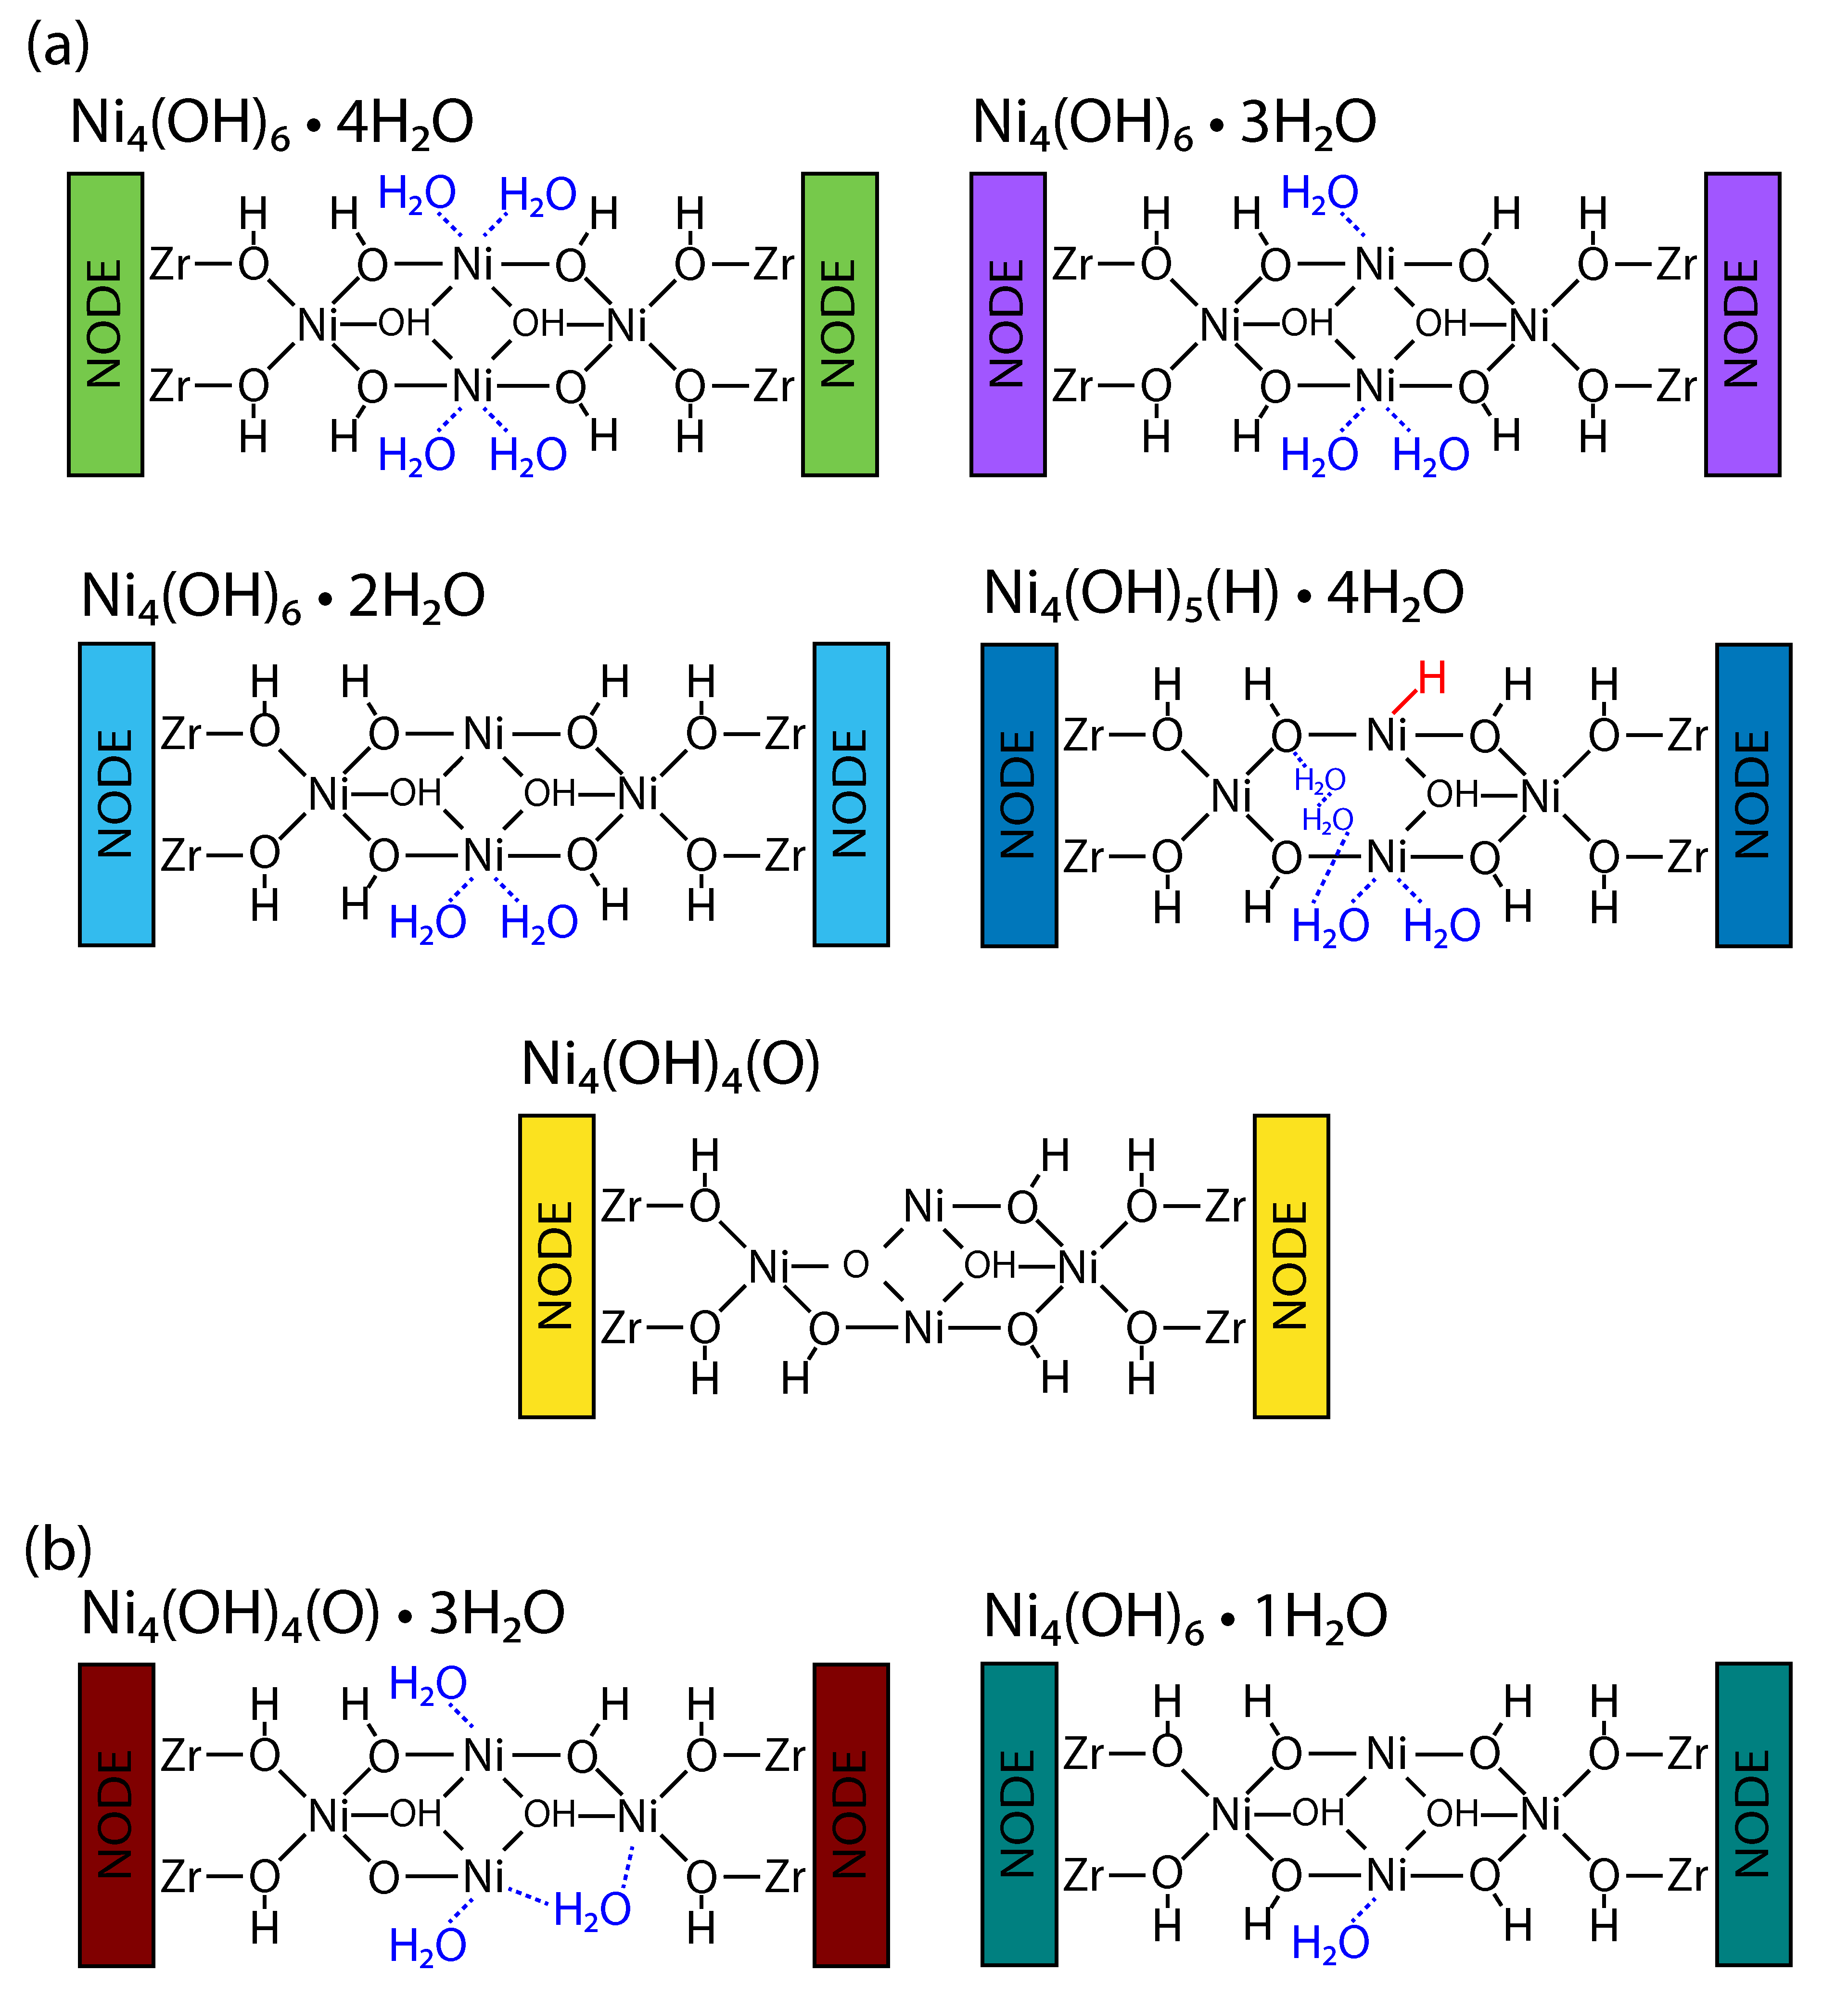
\includegraphics[width=0.75\textwidth]{zi-images/01-Ni-Graphics/2021-MAIN-structure-diagram.png}
    \caption{
    Depiction of key structures considered in this work from (a) \textit{ab initio} thermodynamic modeling structures and (b) select non-thermodynamic minima. The color scheme is the same as in Figures~\ref{fig:phase_diagram_Ni} and \ref{fig:dPDFs-graphic}. All \ce{H2O}s are colored blue, and any Nickel hydride species (\ce{Ni-H}) are colored red. The color scheme is the same as in Figures~\ref{fig:phase_diagram_Ni} and \ref{fig:dPDFs-graphic}.
    }
    \label{fig:Ni-structure-diagram}
\end{figure}

   
To provide molecular-level insight into the ligand environments that could lead to the experimentally observed dPDF spectrum, dPDF spectra for calculated structures with \ce{Ni-O} coordination numbers $\ge$ 4 are shown in Figure~\ref{fig:dPDFs-graphic} (b). We seek those structures that give good agreement with the \ce{Ni-O} and \ce{Ni{\Compactcdots}Ni} peaks seen in the experimental dPDF, since \ldots. For the \ce{Ni-O} peak, reasonable agreement by all structures in Figure~\ref{fig:dPDFs-graphic} is seen with the exception of \ce{Ni4(OH)5(H).4H2O} (blue), which exhibits asymmetric split \ce{Ni-O} peaks instead of a single \ce{Ni-O} peak. From Figure~\ref{fig:Ni-structure-diagram}, this asymmetry is likely caused by asymmetric \ce{Ni-O} distances resulting from coordinated \ce{H2O} ligands that form a bridge across the Ni cluster structure. There is less agreement for the \ce{Ni{\Compactcdots}Ni} peaks. These peaks are split in the experimental dPDF spectrum, suggesting asymmetry, whereas in general, spectra for computed structures exhibit a single \ce{Ni{\Compactcdots}Ni} peak. The two exceptions are \ce{Ni4(OH)4(O)} (yellow), which features a broadened \ce{Ni{\Compactcdots}Ni} peak, and \ce{Ni4(OH)5(H).4H2O} (blue), which features prominent split \ce{Ni{\Compactcdots}Ni} peaks. From Figure~\ref{fig:Ni-structure-diagram}, the broad \ce{Ni{\Compactcdots}Ni} peak in \ce{Ni4(OH)4(O)} (yellow) is likely caused by \ldots. The split peaks in \ce{Ni4(OH)5(H).4H2O} (blue) are likely caused by \ldots. Taken together, the computational results suggest that the synthesized catalyst exhibits a \ce{Ni-O} coordination number similar to those of \ce{Ni4(OH)6.2H2O} (cyan), \ce{Ni4(OH)6.3H2O} (purple), and \ce{Ni4(OH)6.4H2O} (green) and with a ligand environment similar to \ce{Ni4(OH)4(O)} (yellow) and \ce{Ni4(OH)5(H).4H2O} (blue). We hence expect significant \ce{H2O} ligands and asymmetric arrangements of ligands on the Ni ions in the synthesized structure.

% Paragraph about the dPDF of selected structure
In order to provide further molecular-level insight into the ligand environment of Ni-NU-1000, we generated dPDF spectra for the remaining structures in the database (i.e., including those that do not minimize $\Delta F^{(2)}$). The structure that gives the best agreement with experiment is \ce{Ni4(OH)4)(O).3H2O} (red) (Figures~\ref{fig:dPDFs-graphic} (c) and \ref{fig:Ni-structure-diagram} (b)). This structure exhibits a broad \ce{Ni-O} peak that agrees with the experimental dPDF and split \ce{Ni{\Compactcdots}Ni} peaks that show reasonable agreement. The structure exhibits high \ce{Ni} coordination and a mixture of \ce{OH}, \ce{H2O}, and \ce{O} ligands. The ligand environment is highly asymmetric, leading to split \ce{Ni{\Compactcdots}Ni} peaks at distances that closely reasonable those seen in the experimental dPDF, further suggesting that Ni-NU-1000 catalysts have highly asymmetric mixtures of ligands. Analysis of additional structures supports this claim; \hl{see Supporting information Section XX} for further details.

%The observed asymmetries include both diversity in the \ce{Ni} coordination environment (\ce{OH}, \ce{H2O}, \ce{O}) as well as the orientation of certain ligands (mainly, \ce{H2O}). 

%Prior work suggests that a \ce{Ni-H} is the active site in hydrogenation catalysis on a single \ce{Ni} atom.\cite{Li2016sintering, Shabbir2020} Upon exposure to \ce{H2} gas, the Nickel SSHC is thought to dissociate molecular \ce{H2} into atomic \ce{H} with a \ce{Ni-H} forming and the additional \ce{H} atom being adsorbed by one of the \ce{OH} ligands. We explored structures using a similar approach and systematically generated the structures to include \ce{H} (thus forming the \ce{Ni-H} species). Numerous structures in the library of structures contained a \ce{Ni-H}; however, only the \ce{Ni4(OH)5(H).4H2O} (blue) appears on the phase diagram. \citeauthor{Li2016sintering} suggests that the \ce{Ni-H} might exist under a transient state according to EXAFS.\cite{Li2016sintering} Our thermodynamic model supports this claim. While this work does not rule out metal hydrides as active sites, it suggests that other ligands, e.g., \ce{OH} or \ce{H2O} ligands, could participate in the active site for catalysis. The proton (\ce{H}) necessary for hydrogenation could come from either the \ce{OH} or \ce{H2O} ligands with exposure to \ce{H2} gas regenerating these ligands. The lack of a \ce{Ni-H} raises questions about the catalytically active group for the \ce{Ni} metal complex catalyst. 

% Paragraph talking about the Ni...Zr split peaks
The last remaining feature of the dPDFs not yet explored in this work are the \ce{Ni{\Compactcdots}Zr} split peaks seen in the 3.78 {\AA} and 4.08 {\AA} range in the experimental dPDF (Figure~\ref{fig:dPDFs-graphic} (b)). Similar to the \ce{Ni{\Compactcdots}Ni} split peaks, most structures on the phase diagram (Figure~\ref{fig:phase_diagram_Ni}) exhibit a single peak within the experimental range of the \ce{Ni{\Compactcdots}Zr} peaks. The \ce{Ni{\Compactcdots}Zr} distance is from the attachment of the Nickel SSHC to the NU-1000 node. The \ce{Ni} atoms are connected to the \ce{Zr} via \ce{OH} ligands within our models, and the presence of single peaks suggest that \ce{Ni{\Compactcdots}Zr} distances are uniform in our models. To exhibit asymmetry, it is possible that the two \ce{Ni} ions that connect to the \ce{Zr} nodes exhibit different ligand environments. Alternatively, the NU-1000 unit cell could exhibits asymmetry under reaction conditions. 

Interestingly, only one structure comprising a Ni hydride, i.e., structure \ce{Ni4(OH)5(H).4H2O} (blue), appears on the phase diagram, despite the many that were attempted ($\sim$XX structures in our library comprise Ni hydrides). While this structure minimizes the structure free energy under conditions relevant to catalytic hydrogenation, its \ce{Ni-O} coordination number is notably smaller than the synthesized structure. This could mean that Ni hydrides are not relevant under hydrogenation conditions. Alternatively, it could mean that a variety of ligand environments exist on different Ni ion clusters under hydrogenation conditions, and that those comprising hydrides are the active sites in catalytic hydrogenation.

%The only structure exhibiting split \ce{Ni{\Compactcdots}Ni} peaks is structure \ce{Ni4(OH)5(H).4H2O} (blue), which again features the Nickel-hydride (\ce{Ni-H}) and a bridge of hydrogen bonded \ce{H2O}s. However, only one of these peaks aligns with the experimental peak. The other peak is observed at a larger distance.

% From \citeauthor{Ye2017}, the first coordination sphere of the \ce{Ni4} cluster is thought to be comprised of \ce{OH} and \ce{H2O} ligands with \ce{OH} ligands forming links between \ce{Ni} atoms and \ce{H2O} binding on the ``open" sites of the \ce{Ni} ions in the center of the chain.\cite{Ye2017}

% with the \ce{O} ligand coordinating two \ce{Ni} atoms, lacks a prominent \ce{Ni{\Compactcdots}Ni} peak; a broad peak is observed within the experimental regime



% paragraph on the structure with good coordination from the structure diagrams
%Furthermore, the \ce{Ni-O} coordination number of the activated structure is measured to be $\sim$5 when exposed to \ce{H2} gas. We use the following information as a reference during \textit{ab initio} thermodynamic analysis to identify appropriate \ce{H2} and \ce{H2O} chemical potential values. We neglect \ce{Ni-O} coordination numbers below 3.3 because the lack of \ce{Ni-O} coordination suggests these aren't relevant structures, which is confirmed by their dPDFs (\hl{see Supporting Information}). All structures appearing on the phase diagram (Figure~\ref{fig:phase_diagram_Ni}) are located within the \hl{Supporting Information.} The structures from \textit{ab initio} thermodynamic analysis that minimize the free energy expression (Eq. \ref{eq:free-energy-trans}) and exhibit \ce{Ni-O} coordination numbers above 3.3 are shown in Figure~\ref{fig:Ni-structure-diagram} (a). We order the structures according to the \ce{Ni-O} coordination numbers, determined by inspecting the \ce{Ni-O} bond distances within each structure. The exact \ce{Ni-O} coordination numbers are reported on Figure~\ref{fig:phase_diagram_Ni}.

% paragraph about the structures 
%The structures with \ce{Ni-O} coordination above 3.3, ranked from highest to lowest, are structures \ce{Ni4(OH)6.4H2O} (green), \ce{Ni4(OH)6.3H2O} (purple), \ce{Ni4(OH)6.2H2O} (cyan), \ce{Ni4(OH)5(H).4H2O} (blue), \ce{Ni4(OH)4(O)} (yellow), and \ce{Ni4(OH)4.2H2O} (orange). The specific \ce{Ni} ligand environments are presented in Figure~\ref{fig:Ni-structure-diagram} (a), with structures exhibiting different \ce{Ni-O} coordination environments. The structures exhibit different compositions featuring \ce{OH}, \ce{H2O}, \ce{H}, and \ce{O} ligands coordinated to the \ce{Ni} atoms. Structures \ce{Ni4(OH)6.4H2O} (green), \ce{Ni4(OH)6.3H2O} (purple), and \ce{Ni4(OH)6.2H2O} (cyan) are the same base \ce{Ni4(OH)6} structure, but contain different \ce{H2O} content (Figure~\ref{fig:Ni-structure-diagram} (a)). Structure \ce{Ni4(OH)5(H).4H2O} (blue) is unique in that it contains both a Nickel-hydride (\ce{Ni-H}) and a bridge of hydrogen bonded \ce{H2O}s. Structure \ce{Ni4(OH)4(O)} (yellow) is the only structure featuring an \ce{O} ligand on the phase diagram, and structure \ce{Ni4(OH)4.2H2O} (orange) features a loss of \ce{OH} ligands coordinated to three different \ce{Ni} atoms. The diverse ligand coordination environment for \ce{Ni} is captured by the structures appearing on the phase diagram (Figure~\ref{fig:phase_diagram_Ni}). 



% paragraph talking about the dPDF of the structures on the phase diagram with higher coordination
%Our analysis primarily focuses on the \ce{Ni-O} and \ce{Ni{\Compactcdots}Ni} seen in the experimental dPDF (Figure~\ref{fig:dPDFs-graphic} (a)), where we compare the structures with coordination above 4.0 shown in Figure~\ref{fig:dPDFs-graphic} (b). Selecting high \ce{Ni-O} coordination is valid, given the mismatch in peak characteristics for 
%structures with low \ce{Ni-O} (\hl{see Supporting Information}). We observe large deviations in peak positions for both the \ce{Ni-O} peak and the split \ce{Ni{\Compactcdots}Ni} peaks at low coordination. As expected, we observe much better agreement between model structures and the experimental dPDF with structures that feature higher \ce{Ni} coordination. 

 

% Paragraph talking about the asymmetry in ligand environment
%A closer inspection of the split peaks in the experimental dPDF at 3.01 {\AA} and 3.27 {\AA} suggests asymmetry in the \ce{Ni} coordination environments. Most structures appearing on the phase diagram (Figure~\ref{fig:phase_diagram_Ni}) are symmetric in their ligand coordination (as showed by the structures located in Figure~\ref{fig:Ni-structure-diagram} (b)). The symmetry in the ligand environment results in symmetric interatomic distances between the different \ce{Ni} species, thereby leading to single peaks \ce{Ni{\Compactcdots}Ni} instead of multiple \ce{Ni{\Compactcdots}Ni} in the 3.01 {\AA} and 3.27 {\AA} range. Our library included structure with asymmetric \ce{Ni} coordination (\hl{as shown in the Supporting information}; however, these structures were not thermodynamic mimima under any explored conditions in \textit{ab initio} thermodynamic analysis. 

%\section{Discussion}
%%%%%%%%%%%%%%%%%%%%%%%%%%%%%%%%%%%%%%%%%%%%%%%%%%%%%%%%%%%%%%%%%%%%%
%% Discussion
%%%%%%%%%%%%%%%%%%%%%%%%%%%%%%%%%%%%%%%%%%%%%%%%%%%%%%%%%%%%%%%%%%%%%

%In general, the simulated structures tend to give good agreement with the \ce{Ni-O} peak when compared to the experimental peak when considering appropriate \ce{Ni-O} coordination numbers. The \ce{Ni-O} peak corresponds to the first coordination shell of the \ce{Ni} atoms; as long as \ce{OH} and \ce{H2O} ligands are present we observe reasonable agreement between the model and experimental \ce{Ni-O} peak. For the \ce{Ni{\Compactcdots}Ni} split peaks, the local coordination of the \ce{Ni} atoms has more of an influence when comparing the simulated and experimental peaks. The \ce{Ni{\Compactcdots}Ni} peaks are from the second coordination shell of the \ce{Ni} atoms. The \ce{Ni{\Compactcdots}Ni} interatomic distances are more sensitive to the ligand environment of the \ce{Ni} atoms compared to the \ce{Ni-O} interatomic distances. None of the structures from \textit{ab initio} thermodynamic analysis exactly recreate the \ce{Ni{\Compactcdots}Ni} peak positions, with most structures only featuring a single 
%\ce{Ni{\Compactcdots}Ni} peak. Only structure \ce{Ni4(OH)5(H).4H2O} (blue) exhibits the split \ce{Ni{\Compactcdots}Ni} peaks. These findings suggests that our model structures aren't preciously recreating the active site environment seen in the experimental system. 

%We identify alternative structures (e.g., structures that are not thermodynamic mimima under any explored conditions) that show reasonable agreement for both the \ce{Ni-O} peak and \ce{Ni{\Compactcdots}Ni} peaks. The composition of structure \ce{Ni4(OH)4)(O).3H2O} (red) from Figure~\ref{fig:Ni-structure-diagram} (b) is both compositional diverse and contains asymmetric ligand coordination. This structure comprises of \ce{OH} and \ce{H2O} ligands, and additionally includes a \ce{\mu_{2}-O} ligand instead of a \ce{\mu_{2}-OH} ligand. The \ce{Ni} coordination is such that the $\ce{OH}$ and $\ce{O}$  ligands link adjacent two \ce{Ni} atoms. Additionally, an $\ce{H2O}$ ligand occupies the space of a $\ce{OH}$ ligand (i.e., the $\ce{H2O}$ ligand is coordinated to two \ce{Ni} atoms). The alternative structure shows split \ce{Ni{\Compactcdots}Ni} peaks with unequally heights, which differs from what was observed experimentally. 

%Given that the structure dPDF that best agrees with the experimental dPDF contains the compositional diverse (\ce{OH}, \ce{H2O}, and \ce{O} ligands) with asymmetric \ce{H2O} ligands and \ce{O} ligand coordinating two \ce{Ni} atoms) ligand coordination suggests that considering alternative structures is important. Although not as pronounced, this structure also exhibits \ce{Ni{\Compactcdots}Zr} peak splitting. While this structure still does not precisely reproduce the experimental dPDF, \ce{Ni4(OH)4)(O).3H2O} (red) provides clues as to the composition and structure of the \ce{Ni} cluster under catalytic operating conditions. Specifically, this structure is likely to comprise at least four \ce{Ni} atoms with high coordination that involves diverse ligand coordination.



%For example, the experimentally observed \ce{Ni{\Compactcdots}Zr} split peaks could be caused by node distortions (i.e., deformations in the MOF crystalline structure). As presently formulated, our model fails to consider any deformations of the MOF crystalline structure. Our unit cell parameters are fixed throughout the entire simulation. As the unit cell dimensions and shapes are held fixed in our models, our models are better able to capture asymmetry due to different ligand environments, but not due to structural effects of the MOF itself. Possible deviations include different coordinating ligands between the two atoms. We did consider variations to the ligands that coordinate directly to the MOF node (\ce{Zr}) and the Nickel SSHC (\ce{Ni}). However, these structures were not thermodynamic minima under any of the explored conditions.

\section{Conclusions}
%%%%%%%%%%%%%%%%%%%%%%%%%%%%%%%%%%%%%%%%%%%%%%%%%%%%%%%%%%%%%%%%%%%%%
%% Conclusions  
%%%%%%%%%%%%%%%%%%%%%%%%%%%%%%%%%%%%%%%%%%%%%%%%%%%%%%%%%%%%%%%%%%%%%

The rich structural landscape of a \ce{Ni} metal complex is modeled using a combination of dPDF analysis and \textit{ab initio} thermodynamic analysis. We quantify the local structures from modeling using dPDF analysis, and compare our model structures to experimental dPDF for a \ce{Ni} metal complex supported on NU-1000 exposed to \ce{H2} gas. Comparisons with experiments reveal the importance of a high \ce{Ni} coordination environment, which is maintained by coordinated \ce{O}, \ce{OH}, and \ce{H2O} groups to the \ce{Ni} atoms of the cluster. A general trend is that the structures containing more \ce{OH} and \ce{H2O} groups show better agreement to the experimental dPDF in dPDF analysis, with these structures generally appearing on the phase diagram at large \ce{H2O} chemical potentials. This suggests that there is a sufficient \ce{H2O} chemical potential with the MOF, which we are unable to define given that \ce{H2O} is not thought of being present within the system. Further, we identify structures with high \ce{Ni-O} coordination and structural diversity (different \ce{O}, \ce{OH}, and \ce{H2O} ligands). The diverse ligand environment enables asymmetries in the interatomic distances, which enables asymmetries in the \ce{Ni{\Compactcdots}Ni} peaks. Model dPDFs showing the best agreement with the experimental dPDFs feature high coordination and a diverse \ce{Ni-O} coordination environment. Given the diverse structures of the \ce{Ni} cluster, our findings suggest that alternate ligand coordination environments should be considered when modeling SSHCs supported on MOFs. 


\section{References}

%The class makes various changes to the way that references are
%handled.  The class loads \textsf{natbib}, and also the
%appropriate bibliography style.  References can be made using
%the normal method; the citation should be placed before any
%punctuation, as the class will move it if using a superscript
%citation style
%\cite{Mena2000,Abernethy2003,Friedman-Hill2003,EuropeanCommission2008}.
%The use of \textsf{natbib} allows the use of the various citation
%commands of that package: \citeauthor{Abernethy2003} have shown
%something, in \citeyear{Cotton1999}, or as given by
%Ref.~\citenum{Mena2000}.  Long lists of authors will be
%automatically truncated in most article formats, but not in
%supplementary information or reviews \cite{Pople2003}. If you
%encounter problems with the citation macros, please check that
%your copy of \textsf{natbib} is up to date. The demonstration
%database file \texttt{achemso-demo.bib} shows how to complete
%entries correctly. Notice that ``\latin{et al.}'' is auto-formatted
%using the \texttt{\textbackslash latin} command.

%Multiple citations to be combined into a list can be %given as
%a single citation.  This uses the \textsf{mciteplus} %package
%\cite{Johnson1972,*Arduengo1992,*Eisenstein2005,*Arduengo%1994}.
%Citations other than the first of the list should be %indicated
%with a star. If the \textsf{mciteplus} package is not %installed,
%the standard bibliography tools will still work but %starred
%references will be ignored. Individual references can be %referred
%to using \texttt{\textbackslash mciteSubRef}:
%``ref.~\mciteSubRef{Eisenstein2005}''.

%The class also handles notes to be added to the bibliography.  These
%should be given in place in the document \bibnote{This is a note.
%The text will be moved the the references section.  The title of the
%section will change to ``Notes and References''.}.  As with
%citations, the text should be placed before punctuation.  A note is
%also generated if a citation has an optional note.  This assumes that
%the whole work has already been cited: odd numbering will result if
%this is not the case \cite[p.~1]{Cotton1999}.

%%%%%%%%%%%%%%%%%%%%%%%%%%%%%%%%%%%%%%%%%%%%%%%%%%%%%%%%%%%%%%%%%%%%%
%% The "Acknowledgement" section can be given in all manuscript
%% classes.  This should be given within the "acknowledgement"
%% environment, which will make the correct section or running title.
%%%%%%%%%%%%%%%%%%%%%%%%%%%%%%%%%%%%%%%%%%%%%%%%%%%%%%%%%%%%%%%%%%%%%
%\begin{acknowledgement}
%
%\hl{authors would like to thank \ldots''.
%
%The author thanks Mats Dahlgren for version one of \textsf{achemso},
%and Donald Arseneau for the code taken from \textsf{cite} to move
%citations after punctuation. Many users have provided feedback on the
%class, which is reflected in all of the different demonstrations
%shown in this document.}
%
%\end{acknowledgement}

%%%%%%%%%%%%%%%%%%%%%%%%%%%%%%%%%%%%%%%%%%%%%%%%%%%%%%%%%%%%%%%%%%%%%
%% The same is true for Supporting Information, which should use the
%% suppinfo environment.
%%%%%%%%%%%%%%%%%%%%%%%%%%%%%%%%%%%%%%%%%%%%%%%%%%%%%%%%%%%%%%%%%%%%%
%\begin{suppinfo}
%
%\hl{This will usually read something like: ``Experimental procedures and
%characterization data for all new compounds. The class will
%automatically add a sentence pointing to the information on-line:}
%
%\end{suppinfo}

%%%%%%%%%%%%%%%%%%%%%%%%%%%%%%%%%%%%%%%%%%%%%%%%%%%%%%%%%%%%%%%%%%%%%
%% The appropriate \bibliography command should be placed here.
%% Notice that the class file automatically sets \bibliographystyle
%% and also names the section correctly.
%%%%%%%%%%%%%%%%%%%%%%%%%%%%%%%%%%%%%%%%%%%%%%%%%%%%%%%%%%%%%%%%%%%%%
\bibliography{achemso-demo}

\end{document}